\documentclass[11pt,oneside]{article}

\usepackage[a4paper,margin=26mm,headheight=15pt]{geometry}
\usepackage[T1]{fontenc}
\usepackage[utf8]{inputenc}
\IfFileExists{libertinus.sty}{\usepackage{libertinus}}{\usepackage{lmodern}}
\usepackage{microtype}
\usepackage{amsmath,amssymb,amsthm,mathtools,mathrsfs,bm}
\usepackage{booktabs,longtable,tabularx,array,multirow}
\usepackage{graphicx}
\usepackage[dvipsnames]{xcolor}
\usepackage{enumitem}
\usepackage{fancyhdr}
\usepackage{titlesec}
\usepackage[most]{tcolorbox}
\usepackage{listings}
\usepackage{xurl}
\usepackage{hyperref}
\usepackage[nameinlink,noabbrev]{cleveref}

\definecolor{linkblue}{RGB}{24,73,127}
\definecolor{provedgreen}{RGB}{25,105,69}
\definecolor{derivedblue}{RGB}{42,84,133}
\definecolor{frontierorange}{RGB}{155,87,17}
\definecolor{shadegray}{RGB}{246,247,249}
\definecolor{rulegray}{RGB}{192,199,207}
\definecolor{deepviolet}{RGB}{87,55,132}

\hypersetup{
  colorlinks=true,
  linkcolor=linkblue,
  citecolor=deepviolet,
  urlcolor=linkblue,
  pdftitle={Polyphase, Operator, and Jump-Measure Representations of the Fabius--Rvachev System},
  pdfauthor={OpenAI GPT-5.6 Pro, prepared for Vladimir Reshetnikov},
  pdfsubject={Representation atlas, sparse-scale sinc products, multidimensional section integrals, and new Thue--Morse formulas},
  pdfkeywords={Fabius function, Rvachev up-function, Thue-Morse, sinc product, polyphase, q-binomial, Bell polynomial, Bernoulli number, Lambert W}
}

\pagestyle{fancy}
\fancyhf{}
\fancyhead[L]{\small Polyphase representations of the Fabius--Rvachev system}
\fancyhead[R]{\small\nouppercase{\leftmark}}
\fancyfoot[C]{\thepage}
\renewcommand{\headrulewidth}{0.4pt}

\titleformat{\section}{\Large\bfseries\color{linkblue}}{\thesection}{0.72em}{}
\titleformat{\subsection}{\large\bfseries\color{linkblue}}{\thesubsection}{0.65em}{}
\titleformat{\subsubsection}{\normalsize\bfseries\color{provedgreen}}{\thesubsubsection}{0.58em}{}
\setcounter{tocdepth}{2}
\setcounter{secnumdepth}{3}
\numberwithin{equation}{section}
\allowdisplaybreaks[3]
\setlength{\emergencystretch}{3em}
\setlist[itemize]{leftmargin=2em,itemsep=0.25em,topsep=0.45em}
\setlist[enumerate]{leftmargin=2.3em,itemsep=0.25em,topsep=0.45em}

\newtheorem{theorem}{Theorem}[section]
\newtheorem{proposition}[theorem]{Proposition}
\newtheorem{lemma}[theorem]{Lemma}
\newtheorem{corollary}[theorem]{Corollary}
\newtheorem{identity}[theorem]{Identity}
\newtheorem{conjecture}[theorem]{Conjecture}
\newtheorem{problem}[theorem]{Open problem}
\theoremstyle{definition}
\newtheorem{definition}[theorem]{Definition}
\newtheorem{algorithm}[theorem]{Algorithm}
\newtheorem{example}[theorem]{Example}
\theoremstyle{remark}
\newtheorem{remark}[theorem]{Remark}
\newtheorem{warning}[theorem]{Warning}

\newtcolorbox{resultbox}[1][]{
  enhanced,breakable,colback=blue!2,colframe=MidnightBlue!72!black,
  boxrule=0.65pt,arc=1.2mm,left=2mm,right=2mm,top=1.2mm,bottom=1.2mm,
  title={#1},fonttitle=\bfseries
}
\newtcolorbox{statusbox}[1][]{
  enhanced,breakable,colback=gray!4,colframe=gray!62,
  boxrule=0.55pt,arc=1mm,left=2mm,right=2mm,top=1.1mm,bottom=1.1mm,
  title={#1},fonttitle=\bfseries
}
\newtcolorbox{frontierbox}[1][]{
  enhanced,breakable,colback=orange!3,colframe=frontierorange!85!black,
  boxrule=0.65pt,arc=1.2mm,left=2mm,right=2mm,top=1.2mm,bottom=1.2mm,
  title={#1},fonttitle=\bfseries
}

\lstdefinestyle{python}{
  language=Python,
  basicstyle=\ttfamily\small,
  backgroundcolor=\color{shadegray},
  frame=single,
  rulecolor=\color{rulegray},
  columns=fullflexible,
  breaklines=true,
  keepspaces=true,
  showstringspaces=false,
  keywordstyle=\color{linkblue}\bfseries,
  commentstyle=\color{provedgreen},
  stringstyle=\color{frontierorange}
}

\newcommand{\R}{\mathbb R}
\newcommand{\C}{\mathbb C}
\newcommand{\Q}{\mathbb Q}
\newcommand{\N}{\mathbb N}
\newcommand{\Z}{\mathbb Z}
\newcommand{\E}{\mathbb E}
\newcommand{\Prob}{\mathbb P}
\newcommand{\Var}{\operatorname{Var}}
\newcommand{\Cov}{\operatorname{Cov}}
\newcommand{\Law}{\operatorname{Law}}
\newcommand{\Up}{\operatorname{up}}
\newcommand{\sincpi}{\operatorname{sinc}_{\pi}}
\newcommand{\sgn}{\operatorname{sgn}}
\newcommand{\ord}{\operatorname{ord}}
\newcommand{\Res}{\operatorname*{Res}}
\newcommand{\supp}{\operatorname{supp}}
\newcommand{\vtwo}{\nu_2}
\newcommand{\wt}{s_2}
\newcommand{\dd}{\,\mathrm d}
\newcommand{\e}{\mathrm e}
\newcommand{\ii}{\mathrm i}
\newcommand{\bigO}{\mathcal O}
\newcommand{\smallo}{o}
\newcommand{\eps}{\varepsilon}
\newcommand{\qbinom}[3]{\genfrac{[}{]}{0pt}{}{#1}{#2}_{#3}}
\newcommand{\pospart}[1]{\left(#1\right)_{+}}
\newcommand{\jump}[2]{\left[#1\right]_{#2}}
\newcommand{\norm}[1]{\left\lVert#1\right\rVert}
\newcommand{\abs}[1]{\left\lvert#1\right\rvert}
\newcommand{\cF}{\mathcal F}
\newcommand{\cM}{\mathcal M}
\newcommand{\cU}{\mathcal U}
\newcommand{\cG}{\mathcal G}
\newcommand{\cB}{\mathcal B}
\newcommand{\cC}{\mathcal C}
\newcommand{\cR}{\mathcal R}
\newcommand{\cT}{\mathcal T}
\newcommand{\bigast}{\mathop{\text{\Large$\ast$}}\limits}
\newcommand{\statusknown}{\textcolor{deepviolet}{\textsf{K}}}
\newcommand{\statusderived}{\textcolor{derivedblue}{\textsf{D}}}
\newcommand{\statusnew}{\textcolor{provedgreen}{\textsf{N}}}
\newcommand{\statusconj}{\textcolor{frontierorange}{\textsf{C}}}
\newcommand{\repo}{\texttt{ProveIt}}

\title{\bfseries Polyphase, Operator, and Jump-Measure Representations\\[0.25em]
of the Fabius--Rvachev System\\[0.55em]
\large A corpus-aware representation atlas with sparse-scale sinc products,\\
multidimensional section integrals, and new Thue--Morse formulas}
\author{Prepared for Vladimir Reshetnikov\\
\small OpenAI GPT-5.6 Pro}
\date{28 August 2026\\
\small repository snapshot \nolinkurl{19ad531146cda7bc11a206827566db7f5753d5b3}}

\begin{document}
\maketitle

\begin{abstract}
The recursive LaTeX corpus under
\path{Analysis/FabiusFunction/docs} already contains a large fraction of the
modern analytic theory of the Fabius function, its inverse, Rvachev's compactly
supported up-function, the Thue--Morse sequence, dyadic and Gaussian
$q$-binomial arithmetic, sinc products, spectral determinants, Bell--Bernoulli
moment algebra, and periodic Lambert--$W$ endpoint asymptotics.  The purpose of
this report is therefore twofold: first, to organize the existing material as a
single representation atlas; second, to add a complementary layer that was not
located in the audited corpus.

The new organizing object is the sparse-scale Fourier product
\[
 \Psi_r(z)=\prod_{m\ge0}\sincpi\!\left(\frac{z}{2^{rm}}\right),
 \qquad r\in\N_{>0}.
\]
Partitioning the scales of the ordinary Rvachev product modulo $r$ gives the
exact polyphase factorization
\[
 \widehat{\Up}(z)=\prod_{a=0}^{r-1}\Psi_r(z/2^a).
\]
If $g_r$ is the probability density with Fourier image $\Psi_r$, then
\[
 \Up=g_r*(2g_r(2\,\cdot))*\cdots*(2^{r-1}g_r(2^{r-1}\,\cdot)).
\]
This one identity generates cosine, Gamma, canonical-zero, logarithmic-zeta,
hyperbolic-product, cumulant, Bell-polynomial, spectral-zeta, and integral
representations.  The component zero multiplicity is
$1+\lfloor\nu_2(n)/r\rfloor$, and its spectral zeta is
$\zeta(s)/(1-2^{-rs})$.  Mellin analysis shows an exact roots-of-unity
cancellation: the $r$-periodic pole lattice of a sparse component recombines so
that only the ordinary dyadic harmonics survive.

The probability factorization yields a new family of finite-dimensional
representations.  With
$w_r=(1,2^{-1},\ldots,2^{-(r-1)})$ and independent coordinates having density
$g_r$, the Fabius function is both a sublevel-set volume and a parallel
hyperplane section:
\[
 F(x)=\int_{w_r\cdot y\le2x-1}\prod_{a=0}^{r-1}g_r(y_a)\,\dd y
 =\frac1{\norm{w_r}_2}\int_{w_r\cdot y=x-1}
       \prod_{a=0}^{r-1}g_r(y_a)\,\dd\sigma(y).
\]
The equality of a moving volume and a differently placed section is the
multidimensional form of the self-CDF identity $F(x)=\Up(x-1)$.

A second new package extracts the Thue--Morse sequence from analytic data.
Finite sparse box splines $g_{r,N}$ have knots
$x_{r,N,k}=-A_{r,N}+\sum_j b_j(k)2^{-rj}$, and their highest classical
derivative has jumps
\[
 \eps_k=(-1)^{s_2(k)}
 =2^{-r\binom N2}\jump{D^{N-1}g_{r,N}}{x_{r,N,k}}.
\]
Equivalently, the complete signed block is the inverse Fourier transform of a
deconvolution quotient:
\[
 \sum_{k<2^N}\eps_k\delta_{x_{r,N,k}}
 =2^{-r\binom N2}D^N\cF^{-1}\!\left[
   \frac{\Psi_r(z)}{\Psi_r(z/2^{rN})}\right].
\]
Taking the positive and negative Jordan parts gives equally explicit formulas
for the unsigned sequence.  Pairing this measure with high powers gives exact
Bell--Bernoulli formulas for all surviving Thue--Morse power sums and new limit
representations for every moment of $g_r$ and $\Up$.

Finally, convolution is recast as an infinite product of averaging operators,
\[
 \Up=\exp\!\left(
  \sum_{m\ge1}\frac{B_{2m}}{2m(2m)!(1-4^{-m})}D^{2m}
 \right)\delta_0,
\]
with a rigorous polynomial interpretation and a strong-operator
interpretation through uniform averaging.  Commented Python code checks the
polyphase products, Fourier deconvolution, exact power sums, and cumulant
recombination.  Throughout, ``new'' means new relative to the pinned repository
snapshot; no claim of worldwide bibliographic priority is made without a
separate exhaustive literature search.
\end{abstract}

\tableofcontents
\clearpage

\section{Scope, corpus audit, and novelty discipline}
\label{sec:audit}

\subsection{Pinned source boundary}

The branch moved during the audit, so the mathematical source boundary is the
exact commit printed on the title page.  The recursive documentation tree was
classified into five strata:
\begin{enumerate}
\item the primary theorem-backed exposition and mathematical glossary;
\item the living non-formalized frontier synthesis;
\item active thematic reports on Thue--Morse, spectra, arithmetic rays,
      exponent sequences, transforms, inverse sampling, multiresolution, and
      Fourier decay;
\item frozen historical lineages under \path{archive/};
\item imported or corrected primary-paper sources under \path{papers/}.
\end{enumerate}
Every TeX path was included in the recursive inventory.  Superseded or nearly
identical archive revisions were treated through their provenance lineages
rather than counted as independent mathematical discoveries.  The canonical
current descendants were used as the source of record, while targeted
full-corpus searches were made for every proposed new structure.

The most relevant exclusion sources are the primary Fabius--Rvachev synthesis
\cite{repoPrimary}, the unified Thue--Morse atlas \cite{repoAtlas}, the
finite-block calculus \cite{repoFiniteBlock}, the representation-frontier
report \cite{repoRepresentations}, the multiresolution report
\cite{repoMultiresolution}, the inverse/sampling synthesis \cite{repoInverse},
the exponent-sequence synthesis \cite{repoExponents}, and the
spectral-arithmetic synthesis \cite{repoSpectra}.  The imported literature was
also checked, notably Fabius's original probabilistic example, Rvachev's compact
support theory, Arias de Reyna's analytic and arithmetic papers, and the
lacunary-product literature \cite{fabius1966,rvachev1990,arias1982,arias2018,
aistleitner2017}.

\subsection{Status convention}

The report uses four status tags.
\begin{center}
\begin{tabularx}{0.94\textwidth}{@{}cX@{}}
\toprule
Tag & Meaning \\
\midrule
\statusknown & Explicit in the audited repository or classical source; retained to make the atlas usable.\\
\statusderived & A short transform, specialization, or recombination of known material; proved for completeness but not promoted as a substantive novelty.\\
\statusnew & Apparently absent from the pinned TeX corpus; a proof is supplied here.\\
\statusconj & Conjectural or proposed research direction; numerical evidence is identified separately.\\
\bottomrule
\end{tabularx}
\end{center}

\subsection{What is deliberately not claimed as new}

The following substantial structures already occur in the corpus and are
therefore used only as baseline:
\begin{itemize}
\item the probability law of a geometrically weighted uniform series, finite
      atomic and spline approximants, the Fabius/up fold, and quantile transport;
\item the sinc and triangular cosine products, Fourier inversion, critical
      Poisson cosine series, partition of unity, and exact integer-zero jets;
\item exact dyadic values, Gaussian $q$-binomial formulae, Thue--Morse products,
      Prouhet cancellation, Mahler equations, Dirichlet--Mellin theory, and the
      large signed/unsigned formula atlas;
\item sharp Fourier decay, log-periodic fluctuations, arithmetic rays,
      half-integer spectra, cyclotomic traces, spectral determinants, heat
      traces, and Barnes/Gamma dualities;
\item Cauchy--Stieltjes resolvents, logarithmic finite-level resolvents, Jacobi
      and Stieltjes continued fractions, and Fredholm determinant models;
\item Haar, Faber--Schauder, Walsh--Hadamard, beta-mixture, sinc-mixture,
      Fourier--Legendre, and inverse self-sampling representations;
\item integer and fractional integration packages, inverse endpoint reversion,
      Bell-polynomial coefficient calculus, and periodic lower-Lambert
      asymptotics.
\end{itemize}

\begin{statusbox}[Novelty boundary in one sentence]
The new contribution is not another isolated formula for the same sinc product.
It is a modular-scale factorization that simultaneously produces a sparse
Rvachev family, a Mellin alias-cancellation law, multidimensional volume--section
identities, and analytic jump formulas for the signed and unsigned Thue--Morse
sequences.
\end{statusbox}

\section{Normalization and structural dictionary}
\label{sec:normalization}

\subsection{The probability law, the bump, and the bounded function}

Let $(U_n)_{n\ge0}$ be independent random variables uniformly distributed on
$[-1,1]$, and set
\begin{equation}
 X=\sum_{n=0}^{\infty}2^{-n-1}U_n.                         \label{eq:X-series}
\end{equation}
The series converges absolutely almost surely, $X\in[-1,1]$, and its density is
Rvachev's even bump
\begin{equation}
 u(x):=\Up(x),\qquad \int_{-1}^{1}u(x)\,\dd x=1,
 \qquad u(0)=1.                                            \label{eq:u-normalization}
\end{equation}
Let
\begin{equation}
 Y=\frac{X+1}{2}\in[0,1].                                  \label{eq:Y-def}
\end{equation}
The bounded Fabius function is the distribution function of $Y$:
\begin{equation}
 F(x)=\Prob(Y\le x)=\Prob(X\le2x-1),\qquad 0\le x\le1.   \label{eq:F-cdf}
\end{equation}
The special self-similarity of the law gives the stronger pointwise fold
\begin{equation}
 F(x)=u(x-1),\qquad F(1-x)=u(x),\qquad 0\le x\le1.          \label{eq:F-u-fold}
\end{equation}
Thus the same function value is at once a probability of a half-line and a
density value at a different point.

The inverse Fabius function is denoted
\begin{equation}
 G=F^{-1}:(0,1)\longrightarrow(0,1).                       \label{eq:G-def}
\end{equation}
Endpoint totalizations can be added when needed; no ambiguity below depends on
them.

\subsection{Fourier and sinc conventions}

The Fourier transform is
\begin{equation}
 \widehat f(z)=\int_{\R}f(x)\e^{-2\pi\ii zx}\,\dd x,
 \qquad
 f(x)=\int_{\R}\widehat f(z)\e^{2\pi\ii zx}\,\dd z.       \label{eq:Fourier-convention}
\end{equation}
Write
\begin{equation}
 \sincpi(z)=\frac{\sin(\pi z)}{\pi z},\qquad \sincpi(0)=1,
 \qquad \Phi(z)=\widehat u(z).                             \label{eq:sinc-Phi}
\end{equation}
Then
\begin{equation}
 \Phi(z)=\prod_{n=0}^{\infty}\sincpi\!\left(\frac z{2^n}\right),
 \qquad
 \Phi(z)=\sincpi(z)\Phi(z/2).                              \label{eq:Phi-product-scale}
\end{equation}
The moment-generating function is
\begin{equation}
 M(s)=\E\e^{sX}=\Phi\!\left(\frac{\ii s}{2\pi}\right)
 =\prod_{n=0}^{\infty}
   \frac{\sinh(s/2^{n+1})}{s/2^{n+1}}.                    \label{eq:M-product}
\end{equation}

\subsection{Thue--Morse normalizations}

For $k\ge0$, write
\begin{equation}
 \tau(k)=s_2(k)\bmod2\in\{0,1\},
 \qquad
 \eps_k=(-1)^{s_2(k)}=1-2\tau(k).                          \label{eq:TM-normalizations}
\end{equation}
The signed normalization is natural for products, differences, and atomic
measures.  The unsigned normalization is recovered by
\begin{equation}
 \tau(k)=\frac{1-\eps_k}{2}.                               \label{eq:TM-bridge}
\end{equation}

\section{A compact representation atlas}
\label{sec:atlas}

This section records the main representation families already available in the
corpus, plus immediate transforms needed later.  It is intentionally compact:
the detailed novelty begins in \cref{sec:polyphase}.  The tags refer to the
convention of \cref{sec:audit}.

\subsection{Probability, infinite-cube, and distribution representations}

From \eqref{eq:X-series}, for every bounded Borel function $h$,
\begin{align}
 \int_{-1}^{1}h(x)u(x)\,\dd x
 &=\E\,h\!\left(\sum_{n\ge0}2^{-n-1}U_n\right),             \label{eq:prob-test}\\
 F(x)
 &=\int_{[-1,1]^{\N}}\mathbf1_{\{\sum 2^{-n-1}v_n\le2x-1\}}
       \prod_{n\ge0}\frac{\dd v_n}{2}.                   \label{eq:infinite-cube-F}
\end{align}
These are \statusknown.  They immediately imply the quantile-transport formula
\begin{equation}
 \int_0^1 h(G(y))\,\dd y
 =\int_0^1 h(x)\,\dd F(x)
 =\E\,h(Y),                                                \label{eq:quantile-transport}
\end{equation}
again \statusknown.

\subsection{Differential and refinement representations}

The bump satisfies
\begin{equation}
 u'(x)=2\bigl(u(2x+1)-u(2x-1)\bigr),                        \label{eq:u-DDE}
\end{equation}
and $F$ satisfies
\begin{equation}
 F'(x)=2F(2x)\quad(0\le x\le1/2),
 \qquad F(1-x)=1-F(x).                                     \label{eq:F-DDE}
\end{equation}
Together with \eqref{eq:F-u-fold}, these give two useful inverse-derivative
forms:
\begin{equation}
 G'(y)=\frac1{F'(G(y))}
 =\frac1{u'(G(y)-1)}
 =\frac1{2u(2G(y)-1)}.                                     \label{eq:G-prime}
\end{equation}
All are \statusknown.

\subsection{Fourier inversion and CDF inversion}

Rapid decay of $\Phi$ gives
\begin{align}
 u(x)&=\int_{\R}\Phi(z)\e^{2\pi\ii zx}\,\dd z
      =2\int_0^{\infty}\Phi(z)\cos(2\pi zx)\,\dd z,        \label{eq:u-Fourier-inversion}\\
 F(x)&=\int_{\R}\Phi(z)\e^{2\pi\ii z(x-1)}\,\dd z,
      \qquad 0\le x\le1.                                  \label{eq:F-density-inversion}
\end{align}
Applying the Gil--Pelaez inversion formula to $X$ gives the companion CDF form
\begin{equation}
 F(x)=\frac12+\frac1\pi\int_0^{\infty}
       \Phi(z)\frac{\sin(2\pi z(2x-1))}{z}\,\dd z.         \label{eq:F-CDF-inversion}
\end{equation}
The equality of \eqref{eq:F-density-inversion} and
\eqref{eq:F-CDF-inversion} is a Fourier form of the self-CDF identity.
Status: \statusknown/\statusderived.

\subsection{Laplace, Bromwich, and Fourier images of the bounded function}

The Laplace--Stieltjes transform of $F$ is
\begin{equation}
 \int_0^1\e^{sx}\,\dd F(x)=\E\e^{sY}
 =\e^{s/2}M(s/2).                                          \label{eq:F-LS}
\end{equation}
Integration by parts therefore yields, for $s\ne0$,
\begin{equation}
 \int_0^1\e^{sx}F(x)\,\dd x
 =\frac{\e^s-\e^{s/2}M(s/2)}{s},                           \label{eq:F-Laplace}
\end{equation}
with limiting value $1/2$ at $s=0$.  Setting $s=-2\pi\ii\xi$ gives the exact
Fourier image
\begin{equation}
 \widehat{F\mathbf1_{[0,1]}}(\xi)
 =\frac{\e^{-\pi\ii\xi}\Phi(\xi/2)-\e^{-2\pi\ii\xi}}
        {2\pi\ii\xi},                                    \label{eq:F-Fourier}
\end{equation}
again continued by $1/2$ at the origin.  Conversely, for $c>0$ and
$0<x<1$,
\begin{equation}
 F(x)=\frac1{2\pi\ii}\int_{c-\ii\infty}^{c+\ii\infty}
       \frac{\e^{s(x-1/2)}}{s}M(s/2)\,\dd s.               \label{eq:F-Bromwich}
\end{equation}
These formulas are \statusknown or immediate one-line transforms of known
identities.

\subsection{Product, canonical-zero, and Gamma representations}

The audited corpus contains the following equivalent products:
\begin{align}
 \Phi(z)
 &=\prod_{n=0}^{\infty}\sincpi(z/2^n),                     \label{eq:atlas-sinc}\\
 &=\prod_{m=1}^{\infty}\cos(\pi z/2^m)^m,                  \label{eq:atlas-cos}\\
 &=\prod_{n=1}^{\infty}\left(1-\frac{z^2}{n^2}\right)^{1+\vtwo(n)}, \label{eq:atlas-canonical}\\
 &=\prod_{n=0}^{\infty}
   \frac1{\Gamma(1+z/2^n)\Gamma(1-z/2^n)}.                \label{eq:atlas-gamma}
\end{align}
Thus the nonzero integer $n$ is a zero of order $1+\vtwo(n)$.  The local
logarithmic series is
\begin{equation}
 \log\Phi(z)=-\sum_{m=1}^{\infty}
 \frac{\zeta(2m)}{m(1-4^{-m})}z^{2m},\qquad |z|<1,          \label{eq:atlas-log-zeta}
\end{equation}
and the meromorphic logarithmic derivative is
\begin{equation}
 \frac{\Phi'(z)}{\Phi(z)}
 =-2z\sum_{n=1}^{\infty}\frac{1+\vtwo(n)}{n^2-z^2}.        \label{eq:atlas-log-derivative}
\end{equation}
Status: \statusknown.

\subsection{Moments, cumulants, and Bell--Bernoulli series}

Writing
\begin{equation}
 \log M(s)=\sum_{m\ge1}\kappa_{2m}\frac{s^{2m}}{(2m)!},    \label{eq:cumulant-def}
\end{equation}
comparison with \eqref{eq:M-product} gives
\begin{equation}
 \kappa_{2m}=\frac{B_{2m}}{2m(1-4^{-m})},
 \qquad \kappa_{2m+1}=0.                                  \label{eq:full-cumulants}
\end{equation}
Hence
\begin{equation}
 \mu_n:=\int x^n u(x)\,\dd x
 =\cB_n(\kappa_1,\ldots,\kappa_n),                         \label{eq:Bell-moments}
\end{equation}
where $\cB_n$ is the complete exponential Bell polynomial.  In particular
\begin{equation}
 \mu_2=\frac19,\qquad \mu_4=\frac{19}{675},\qquad
 \kappa_4=-\frac2{225}.                                   \label{eq:first-moments}
\end{equation}
Status: \statusknown.

\subsection{Finite splines, Poisson series, and multiresolution forms}

The corpus supplies finite uniform-convolution splines whose coefficients are
Thue--Morse signs, critical Poisson cosine series on $[-1,1]$, exact partition
of unity, Fourier--Legendre expansions, and rational Haar, Walsh, and
Faber--Schauder systems.  Representative formulas are
\begin{align}
 u(x)&=\frac12+\sum_{k\ge0}\Phi(k+\tfrac12)
                 \cos((2k+1)\pi x),                       \label{eq:critical-cosine}\\
 \sum_{j\in\Z}u(x-j)&=1,                                  \label{eq:partition-unity}
\end{align}
with the convergence and endpoint conventions established in the primary
source.  The multiresolution report expresses the same function as limits of
exact rational step mixtures, Haar details, Walsh finite products, Bernstein
beta mixtures, and inverse-quantile sinc mixtures \cite{repoMultiresolution}.
Status: \statusknown.

\subsection{Resolvent and determinant forms}

Let
\begin{equation}
 R(z)=\int_{-1}^{1}\frac{u(x)}{z-x}\,\dd x,
 \qquad z\in\C\setminus[-1,1].                             \label{eq:Cauchy-transform}
\end{equation}
Then
\begin{equation}
 R(z)=\sum_{n=0}^{\infty}\frac{\mu_n}{z^{n+1}}             \label{eq:R-moment-series}
\end{equation}
for $|z|>1$, and the representation-frontier report derives a logarithmic
fixed point, a Thue--Morse derivative tree, finite logarithmic resolvents, and
the Jacobi continued fraction of $R$ \cite{repoRepresentations}.  Likewise
\eqref{eq:atlas-canonical} is the Fredholm determinant
\begin{equation}
 \Phi(z)=\det(I-z^2T),                                     \label{eq:Fredholm}
\end{equation}
where $T$ is diagonal with eigenvalue $n^{-2}$ repeated $1+\vtwo(n)$ times.
Status: \statusknown.

\begin{statusbox}[Transition]
The formulas above are a map, not the claimed contribution.  The remainder of
the report introduces a decomposition by congruence classes of the scale index.
It simultaneously refines the Fourier product, the probability law, the zero
divisor, the Mellin pole lattice, the finite splines, and the Thue--Morse
coefficient measure.
\end{statusbox}

\section{Polyphase factorization by scale classes}
\label{sec:polyphase}

\subsection{Sparse-scale products and laws}

Fix an integer $r\ge1$ and put
\begin{equation}
 q_r=2^{-r},\qquad
 \Psi_r(z)=\prod_{m=0}^{\infty}\sincpi(q_r^m z).            \label{eq:Psi-def}
\end{equation}
Let $Z_r$ be the random series
\begin{equation}
 Z_r=\sum_{m=0}^{\infty}\frac{q_r^m}{2}U_m,                \label{eq:Zr-series}
\end{equation}
where the $U_m$ are independent uniform variables on $[-1,1]$.  Its support
radius is
\begin{equation}
 A_r=\frac1{2(1-q_r)},                                     \label{eq:Ar}
\end{equation}
and its density is denoted $g_r$.  Then
\begin{equation}
 \widehat{g_r}(z)=\Psi_r(z),
 \qquad \supp g_r=[-A_r,A_r].                              \label{eq:gr-Fourier-support}
\end{equation}
The generic geometrically weighted uniform law is part of the repository
baseline.  What is new here is its use as a polyphase factor of the ordinary
Rvachev law.

\begin{theorem}[Polyphase product and convolution factorization]
\label{thm:polyphase-main}
For every integer $r\ge1$,
\begin{equation}
 \boxed{\displaystyle
 \Phi(z)=\prod_{a=0}^{r-1}\Psi_r(z/2^a).}                  \label{eq:polyphase-product}
\end{equation}
Equivalently, if
\begin{equation}
 g_{r,a}(x)=2^a g_r(2^a x)                                 \label{eq:scaled-gr}
\end{equation}
 is the density of $2^{-a}Z_r$, then
\begin{equation}
 \boxed{\displaystyle
 u=g_{r,0}*g_{r,1}*\cdots*g_{r,r-1}.}                       \label{eq:polyphase-convolution}
\end{equation}
In random-variable form,
\begin{equation}
 X\overset{d}=\sum_{a=0}^{r-1}2^{-a}Z_r^{(a)},              \label{eq:polyphase-random}
\end{equation}
where the $Z_r^{(a)}$ are independent copies of $Z_r$.
\end{theorem}

\begin{proof}
Every nonnegative integer has a unique decomposition $n=a+rm$ with
$0\le a<r$ and $m\ge0$.  Therefore
\[
 \prod_{n\ge0}\sincpi(z/2^n)
 =\prod_{a=0}^{r-1}\prod_{m\ge0}
   \sincpi\!\left(\frac{z}{2^{a+rm}}\right)
 =\prod_{a=0}^{r-1}\Psi_r(z/2^a).
\]
The products converge locally uniformly, so regrouping is legitimate.  The
Fourier transform of $g_{r,a}$ is $\Psi_r(z/2^a)$; multiplication of the
transforms gives \eqref{eq:polyphase-convolution}.  The random-series identity
is the same partition of the summands of \eqref{eq:X-series}.
\end{proof}

\begin{remark}
The support radii add exactly:
\begin{equation}
 \sum_{a=0}^{r-1}2^{-a}A_r
 =\frac{1}{2(1-2^{-r})}\sum_{a=0}^{r-1}2^{-a}=1.            \label{eq:support-adds}
\end{equation}
Thus no slack is introduced by the factorization.
\end{remark}

\begin{example}[The even--odd scale split]
For $r=2$,
\begin{equation}
 \Phi(z)=\Psi_2(z)\Psi_2(z/2),
 \qquad
 u=g_2*(2g_2(2\,\cdot)),                                   \label{eq:r2-factorization}
\end{equation}
where $g_2$ is supported on $[-2/3,2/3]$.  One factor contains scales
$1,1/4,1/16,\ldots$ in the full widths; the other contains the intervening
scales after one dyadic contraction.
\end{example}

\subsection{A sparse Rvachev differential equation}

The product \eqref{eq:Psi-def} satisfies
\begin{equation}
 \Psi_r(z)=\sincpi(z)\Psi_r(q_rz).                          \label{eq:Psi-refinement}
\end{equation}
The random fixed point is
\begin{equation}
 Z_r\overset{d}=\frac{U}{2}+q_rZ_r',                        \label{eq:Zr-fixed-point}
\end{equation}
with independent $U\sim\operatorname{Unif}[-1,1]$ and
$Z_r'\overset d=Z_r$.

\begin{proposition}[Sparse-scale Rvachev equation]
\label{prop:sparse-DDE}
The density $g_r$ obeys
\begin{align}
 g_r(x)
 &=\int_{2^rx-2^{r-1}}^{2^rx+2^{r-1}}g_r(t)\,\dd t,        \label{eq:gr-integral-equation}\\
 g_r'(x)
 &=2^r\bigl(g_r(2^rx+2^{r-1})-g_r(2^rx-2^{r-1})\bigr).     \label{eq:gr-DDE}
\end{align}
For $r=1$ this is the ordinary Rvachev equation.
\end{proposition}

\begin{proof}
Condition on $U/2$ in \eqref{eq:Zr-fixed-point}.  The density of $q_rZ_r'$ is
$q_r^{-1}g_r(\cdot/q_r)$, hence
\[
 g_r(x)=\int_{-1/2}^{1/2}q_r^{-1}
 g_r\!\left(\frac{x-y}{q_r}\right)\dd y.
\]
The substitution $t=(x-y)/q_r$ gives
\eqref{eq:gr-integral-equation}; differentiation gives
\eqref{eq:gr-DDE}.
\end{proof}

\subsection{Cosine, Gamma, canonical-zero, and logarithmic forms}

The sparse product has a complete set of analogues of the ordinary Rvachev
representations.

\begin{theorem}[Equivalent products for the sparse component]
\label{thm:Psi-products}
For every $r\ge1$,
\begin{align}
 \Psi_r(z)
 &=\prod_{m=0}^{\infty}\sincpi(z/2^{rm}),                  \label{eq:Psi-sinc}\\
 &=\prod_{n=1}^{\infty}
   \cos(\pi z/2^n)^{1+\lfloor(n-1)/r\rfloor},              \label{eq:Psi-cos}\\
 &=\prod_{n=1}^{\infty}
   \left(1-\frac{z^2}{n^2}\right)^{1+\lfloor\vtwo(n)/r\rfloor}, \label{eq:Psi-canonical}\\
 &=\prod_{m=0}^{\infty}
   \frac1{\Gamma(1+z/2^{rm})\Gamma(1-z/2^{rm})}.           \label{eq:Psi-gamma}
\end{align}
For $|z|<1$,
\begin{equation}
 \log\Psi_r(z)
 =-\sum_{j=1}^{\infty}
   \frac{\zeta(2j)}{j(1-2^{-2rj})}z^{2j}.                 \label{eq:Psi-log-zeta}
\end{equation}
Away from its integer zeros,
\begin{equation}
 \frac{\Psi_r'(z)}{\Psi_r(z)}
 =-2z\sum_{n=1}^{\infty}
   \frac{1+\lfloor\vtwo(n)/r\rfloor}{n^2-z^2}.            \label{eq:Psi-logderivative}
\end{equation}
\end{theorem}

\begin{proof}
The sinc and Gamma forms follow from
$\sincpi w=(\Gamma(1+w)\Gamma(1-w))^{-1}$.  Expanding each sinc by
$\sincpi w=\prod_{j\ge1}\cos(\pi w/2^j)$, a fixed cosine at scale $2^{-n}$
occurs once for each $m\ge0$ with $rm<n$, giving
$1+\lfloor(n-1)/r\rfloor$ copies.  Expanding instead by Euler's sine product,
a zero at a nonzero integer $n$ receives one copy for each $m$ with
$rm\le\vtwo(n)$, hence multiplicity $1+\lfloor\vtwo(n)/r\rfloor$.
The logarithmic series follows from
\(
 \log\sincpi z=-\sum_{j\ge1}\zeta(2j)z^{2j}/j
\)
and a geometric sum.  Logarithmic differentiation of the canonical product
gives \eqref{eq:Psi-logderivative}.
\end{proof}

\begin{corollary}[Exact splitting of the integer zero divisor]
\label{cor:zero-divisor-split}
Let $v=\vtwo(n)$.  The zero order $1+v$ of $\Phi$ at $n\ne0$ decomposes as
\begin{equation}
 1+v=\sum_{a=0}^{r-1}
 \mathbf1_{a\le v}\left(1+\left\lfloor\frac{v-a}{r}\right\rfloor\right). \label{eq:valuation-split}
\end{equation}
The $a$th summand is the order contributed by $\Psi_r(z/2^a)$.
\end{corollary}

\begin{proof}
The right side counts pairs $(a,m)$ satisfying
$0\le a<r$, $m\ge0$, and $a+rm\le v$.  Uniqueness of Euclidean division
identifies these pairs with the integers $0,1,\ldots,v$.
\end{proof}

\subsection{Spectral zeta and determinant splitting}

Let
\begin{equation}
 m_r(n)=1+\left\lfloor\frac{\vtwo(n)}r\right\rfloor.        \label{eq:mr-def}
\end{equation}
The zero divisor of $\Psi_r$ has spectral zeta
\begin{equation}
 \mathcal Z_r(s)=\sum_{n\ge1}\frac{m_r(n)}{n^s}.            \label{eq:Zr-def}
\end{equation}

\begin{proposition}[Sparse spectral zeta]
\label{prop:sparse-spectral-zeta}
For $\Re s>1$,
\begin{equation}
 \boxed{\displaystyle
 \mathcal Z_r(s)=\frac{\zeta(s)}{1-2^{-rs}}.}               \label{eq:sparse-spectral-zeta}
\end{equation}
Moreover the scaled factors satisfy the exact recombination
\begin{equation}
 \sum_{a=0}^{r-1}2^{-as}\mathcal Z_r(s)
 =\frac{\zeta(s)}{1-2^{-s}},                               \label{eq:spectral-zeta-recombine}
\end{equation}
which is the spectral zeta of $\Phi$.
\end{proposition}

\begin{proof}
Each factor $\sincpi(z/2^{rm})$ contributes one zero at every nonzero multiple
of $2^{rm}$.  Therefore
\[
 \mathcal Z_r(s)
 =\sum_{m\ge0}\sum_{k\ge1}(2^{rm}k)^{-s}
 =\zeta(s)\sum_{m\ge0}2^{-rms}.
\]
Scaling the zeros by $2^a$ multiplies their zeta contribution by $2^{-as}$.
The finite geometric sum cancels $1-2^{-rs}$.
\end{proof}

In particular,
\begin{equation}
 \Psi_r(z)=\det(I-z^2T_r),                                  \label{eq:Psi-determinant}
\end{equation}
where $T_r$ has eigenvalue $n^{-2}$ repeated $m_r(n)$ times.  The ordinary
Rvachev determinant is the direct-sum product of the $r$ scaled component
operators.

\subsection{Hyperbolic products, cumulants, and Bell polynomials}

The component moment-generating function is
\begin{equation}
 M_r(s)=\E\e^{sZ_r}
 =\Psi_r\!\left(\frac{\ii s}{2\pi}\right)
 =\prod_{m=0}^{\infty}
   \frac{\sinh(s/2^{rm+1})}{s/2^{rm+1}}.                   \label{eq:Mr-product}
\end{equation}

\begin{theorem}[Sparse cumulants and exact recombination]
\label{thm:sparse-cumulants}
The component cumulants are
\begin{equation}
 \kappa_{2j}^{(r)}
 =\frac{B_{2j}}{2j(1-2^{-2rj})},
 \qquad \kappa_{2j+1}^{(r)}=0.                             \label{eq:sparse-cumulants}
\end{equation}
The $2j$th cumulant of the polyphase sum
\eqref{eq:polyphase-random} is
\begin{equation}
 \sum_{a=0}^{r-1}2^{-2aj}\kappa_{2j}^{(r)}
 =\frac{B_{2j}}{2j(1-2^{-2j})}=\kappa_{2j}.                \label{eq:cumulant-recombine}
\end{equation}
Consequently
\begin{equation}
 \mu_n^{(r)}:=\E Z_r^n
 =\cB_n\bigl(\kappa_1^{(r)},\ldots,\kappa_n^{(r)}\bigr).   \label{eq:sparse-Bell-moments}
\end{equation}
\end{theorem}

\begin{proof}
Use
\[
 \log\frac{\sinh x}{x}
 =\sum_{j\ge1}\frac{2^{2j-1}B_{2j}}{j(2j)!}x^{2j}
\]
in \eqref{eq:Mr-product} and sum the resulting geometric progression.  The
scaling law for cumulants and the finite geometric sum give
\eqref{eq:cumulant-recombine}.  The Bell-polynomial relation between moments
and cumulants is standard.
\end{proof}

The first component values are
\begin{equation}
 \Var Z_r=\frac1{12(1-2^{-2r})},
 \qquad
 \kappa_4^{(r)}=-\frac1{120(1-2^{-4r})}.                   \label{eq:sparse-first-cumulants}
\end{equation}
For $r=2$, for example,
\begin{equation}
 \kappa_2^{(2)}=\frac4{45},\qquad
 \kappa_4^{(2)}=-\frac{32}{3825}.                          \label{eq:r2-cumulants}
\end{equation}
The weighted sum of the two dilated cumulants recovers $1/9$ and $-2/225$.

\begin{resultbox}[Contribution I: one object, many representations]
The sparse product $\Psi_r$ is simultaneously a Fourier image, a Gamma product,
a cosine product with staircase exponents, a canonical product with quotient
valuation multiplicities, a Fredholm determinant, a hyperbolic moment product,
and the transform of a sparse Rvachev density.  Its $r$ dyadic dilates multiply
or convolve to the classical object.  This modular-scale package was not found
as such in the pinned corpus.
\end{resultbox}

\section{Mellin alias cancellation and log-periodic phases}
\label{sec:mellin-polyphase}

The polyphase identity does more than regroup convergent products.  It explains
how the denser dyadic pole lattice is synthesized from a sparse one.

\subsection{A general harmonic-sum lemma}

Let $h:(0,\infty)\to\C$ be such that its Mellin transform
\begin{equation}
 H(s)=\int_0^{\infty}h(t)t^{s-1}\,\dd t                     \label{eq:H-Mellin}
\end{equation}
exists in a vertical strip with $\Re s<0$.  Define
\begin{equation}
 L_r(t)=\sum_{m=0}^{\infty}h(2^{-rm}t).                     \label{eq:Lr-harmonic}
\end{equation}
When necessary, polynomial or logarithmic principal parts are subtracted before
applying this statement, exactly as in standard Mellin analysis of harmonic
sums \cite{flajolet1995}.

\begin{theorem}[Polyphase Mellin cancellation]
\label{thm:Mellin-cancellation}
In every common strip of absolute convergence,
\begin{align}
 \cM[L_r](s)&=\frac{H(s)}{1-2^{rs}},                        \label{eq:Mellin-Lr}\\
 L_1(t)&=\sum_{a=0}^{r-1}L_r(2^{-a}t),                      \label{eq:L1-polyphase}\\
 \cM[L_1](s)&=\frac{H(s)}{1-2^s}.                          \label{eq:Mellin-L1}
\end{align}
At a pole
\begin{equation}
 s_k=\frac{2\pi\ii k}{r\log2}                              \label{eq:sparse-pole-lattice}
\end{equation}
created by $1-2^{rs}$, the scale-sum multiplier is
\begin{equation}
 \sum_{a=0}^{r-1}2^{as_k}
 =\sum_{a=0}^{r-1}\e^{2\pi\ii ka/r}
 =\begin{cases}r,&r\mid k,\\0,&r\nmid k.
 \end{cases}                                               \label{eq:roots-unity-cancel}
\end{equation}
Thus recombination cancels every sparse harmonic except every $r$th one.
\end{theorem}

\begin{proof}
For one term, $t=2^{rm}u$ gives
\[
 \int_0^{\infty}h(2^{-rm}t)t^{s-1}\,\dd t=2^{rms}H(s).
\]
Summation yields \eqref{eq:Mellin-Lr}.  Euclidean division of the scale index
gives \eqref{eq:L1-polyphase}; the Mellin transform of $L_r(2^{-a}t)$ is
$2^{as}\cM[L_r](s)$.  The finite geometric numerator cancels
$1-2^{rs}$ and gives \eqref{eq:Mellin-L1}.  Evaluating the numerator on the
pole lattice gives the roots-of-unity sum.
\end{proof}

\subsection{Application to logarithmic Fourier and Laplace products}

Take, after the usual local regularization,
\begin{equation}
 h(t)=\log\sincpi(t)
 \quad\text{or}\quad
 h(t)=\log\frac{\sinh(t/2)}{t/2}.                           \label{eq:Mellin-kernels}
\end{equation}
Then $L_r$ is respectively $\log\Psi_r$ or $\log M_r$.  The component has a
logarithmic-scale pole lattice with fundamental period $r\log2$; the product of
its $r$ dyadic dilates retains only the harmonics compatible with period
$\log2$.  This is the Mellin-side analogue of
\eqref{eq:valuation-split} and \eqref{eq:cumulant-recombine}.

\begin{corollary}[Periodic coefficient filter]
\label{cor:periodic-filter}
Suppose the regularized asymptotic expansion of a sparse component contains a
Fourier series in the logarithmic phase
\begin{equation}
 P_r(\theta)=\sum_{k\in\Z}c_k\e^{2\pi\ii k\theta/r}.        \label{eq:Pr-phase}
\end{equation}
Then the corresponding coefficient after polyphase recombination is obtained
by the exact projector
\begin{equation}
 P_1(\theta)=\sum_{a=0}^{r-1}P_r(\theta-a)
 =r\sum_{\ell\in\Z}c_{r\ell}\e^{2\pi\ii\ell\theta}.       \label{eq:phase-projector}
\end{equation}
\end{corollary}

\begin{remark}
The existing Fourier-decay campaign identifies nontrivial orbit-dependent and
periodic behavior of the full product.  The theorem above does not replace that
analysis.  It factors its periodic data into a sparse phase and an exact cyclic
projection, suggesting a new way to compute or certify the fluctuation by
working at the longer period $r\log2$ and then filtering.
\end{remark}

\begin{resultbox}[Contribution II: Mellin polyphase projector]
Partitioning the product by scale residues induces a literal roots-of-unity
filter on Mellin residues.  Zero multiplicities, cumulants, and log-periodic
asymptotic harmonics are three manifestations of the same finite cyclic
projection.
\end{resultbox}

\section{Multidimensional volume and section representations}
\label{sec:sections}

The polyphase random decomposition turns the one-dimensional self-CDF identity
into a relation between two different geometric operations on the same product
density: integration over a half-space and integration over a parallel
hyperplane.

\subsection{Radon notation and the product density}

Let
\begin{equation}
 w_r=(1,2^{-1},\ldots,2^{-(r-1)})\in\R^r,
 \qquad
 p_r(y)=\prod_{a=0}^{r-1}g_r(y_a).                         \label{eq:wr-pr}
\end{equation}
For an integrable function $p$ on $\R^r$, define its cumulative and ordinary
Radon transforms in direction $w\ne0$ by
\begin{align}
 \cC_wp(t)&=\int_{w\cdot y\le t}p(y)\,\dd y,              \label{eq:cumulative-Radon}\\
 \cR_wp(t)&=\frac1{\norm w_2}
   \int_{w\cdot y=t}p(y)\,\dd\sigma_{r-1}(y).             \label{eq:Radon-def}
\end{align}
The coarea formula gives $(\cC_wp)'=\cR_wp$ at every continuity point.
For the smooth compactly supported density $p_r$, this holds everywhere.

\begin{theorem}[Polyphase Radon representation]
\label{thm:Radon-representation}
For every $r\ge1$ and every $t\in\R$,
\begin{equation}
 \boxed{\displaystyle
 u(t)=\cR_{w_r}p_r(t),
 \qquad
 \Prob(X\le t)=\cC_{w_r}p_r(t).}                          \label{eq:u-Radon}
\end{equation}
Consequently, for $0\le x\le1$,
\begin{equation}
 \boxed{\displaystyle
 F(x)=\cC_{w_r}p_r(2x-1)=\cR_{w_r}p_r(x-1).}              \label{eq:F-volume-section}
\end{equation}

a relation between a half-space volume at level $2x-1$ and a parallel section
at level $x-1$.
\end{theorem}

\begin{proof}
By \cref{thm:polyphase-main}, the linear form
$w_r\cdot(Z_r^{(0)},\ldots,Z_r^{(r-1)})$ has the same law as $X$.
Its distribution function is therefore the cumulative Radon transform in
\eqref{eq:u-Radon}.  The coarea formula identifies its density with the
ordinary Radon transform.  Substitute the defining relation
$F(x)=\Prob(X\le2x-1)$ and the self-CDF identity $F(x)=u(x-1)$.
\end{proof}

\begin{remark}
At $r=1$, \eqref{eq:F-volume-section} is exactly the one-dimensional identity
\[
 \int_{-\infty}^{2x-1}u(t)\,\dd t=u(x-1).
\]
For $r>1$, the same identity becomes genuinely multidimensional: the left side
is an $r$-dimensional sublevel volume, while the right side is a weighted
$(r-1)$-dimensional slice.
\end{remark}

\subsection{Coordinate integral forms}

Let
\begin{equation}
 H_r(t)=\int_{-\infty}^{t}g_r(v)\,\dd v                    \label{eq:Hr-cdf}
\end{equation}
be the CDF of the sparse component.  Eliminating the last coordinate in the
half-space and in the hyperplane gives two explicit $(r-1)$-fold integrals.

\begin{corollary}[Volume--section integral pair]
\label{cor:coordinate-section}
For $r\ge2$ and $0\le x\le1$,
\begin{align}
 F(x)
 &=\int_{\R^{r-1}}
   \left(\prod_{a=0}^{r-2}g_r(y_a)\right)
   H_r\!\left(2^{r-1}\left(2x-1-
      \sum_{a=0}^{r-2}2^{-a}y_a\right)\right)\dd y,       \label{eq:F-volume-coordinates}\\
 F(x)
 &=2^{r-1}\int_{\R^{r-1}}
   \left(\prod_{a=0}^{r-2}g_r(y_a)\right)
   g_r\!\left(2^{r-1}\left(x-1-
      \sum_{a=0}^{r-2}2^{-a}y_a\right)\right)\dd y.       \label{eq:F-section-coordinates}
\end{align}
Both integrals are effectively over a compact box because $g_r$ is compactly
supported.
\end{corollary}

\begin{proof}
In the volume formula, condition on $y_0,\ldots,y_{r-2}$ and solve the inequality
for $y_{r-1}$.  In the section formula, solve
$w_r\cdot y=x-1$ for the last coordinate.  The Jacobian is $2^{r-1}$.
\end{proof}

For the first nontrivial split $r=2$, writing $H_2$ for the CDF of $g_2$,
\begin{align}
 F(x)
 &=\int_{\R}g_2(y)H_2(4x-2-2y)\,\dd y,                    \label{eq:r2-volume}\\
 &=2\int_{\R}g_2(y)g_2(2x-2-2y)\,\dd y.                  \label{eq:r2-section}
\end{align}
Thus an integral involving the CDF of $g_2$ at one affine scale equals an
integral involving its density at another.

\subsection{A geometric representation of the inverse Fabius function}

The preceding theorem also gives an implicit representation of $G=F^{-1}$ that
uses only one fixed product density and moving parallel hyperplanes.

\begin{corollary}[Two-level geometry of the quantile]
\label{cor:inverse-geometry}
For $0<y<1$, the unique $x=G(y)$ is characterized by
\begin{equation}
 \boxed{\displaystyle
 \cC_{w_r}p_r(2x-1)=\cR_{w_r}p_r(x-1)=y.}                 \label{eq:G-two-level}
\end{equation}
Its derivative is the reciprocal of a third section:
\begin{equation}
 \boxed{\displaystyle
 G'(y)=\frac1{2\cR_{w_r}p_r(2G(y)-1)}.}                   \label{eq:G-Radon-derivative}
\end{equation}
Equivalently, the same product density has section mass $y$ at level $G(y)-1$,
while the section at level $2G(y)-1$ controls the quantile elasticity.
\end{corollary}

\begin{proof}
Equation \eqref{eq:G-two-level} is \eqref{eq:F-volume-section} with $x=G(y)$.
Since $F'(x)=2u(2x-1)$, the inverse-function theorem and
\eqref{eq:u-Radon} give \eqref{eq:G-Radon-derivative}.
\end{proof}

The quantile-transport transform becomes, for every integrable test function
$h$,
\begin{equation}
 \int_0^1h(G(y))\,\dd y
 =\int_{\R^r}h\!\left(\frac{1+w_r\cdot z}{2}\right)
   p_r(z)\,\dd z.                                         \label{eq:G-product-cube}
\end{equation}
In particular,
\begin{equation}
 \int_0^1\e^{sG(y)}\,\dd y
 =\e^{s/2}\prod_{a=0}^{r-1}M_r(s/2^{a+1}),                \label{eq:G-polyphase-MGF}
\end{equation}
which reduces, by cumulant recombination, to
$\e^{s/2}M(s/2)$.

\subsection{Polyphase transforms of the bounded Fabius function}

Substitution of \eqref{eq:polyphase-product} into the transform formulas of
\cref{sec:atlas} gives product--integral representations involving only the
sparse component:
\begin{align}
 F(x)
 &=2\int_0^\infty
   \left(\prod_{a=0}^{r-1}\Psi_r(z/2^a)\right)
   \cos(2\pi z(x-1))\,\dd z,                              \label{eq:F-polyphase-cosine-integral}\\
 F(x)
 &=\frac12+\frac1\pi\int_0^\infty
   \left(\prod_{a=0}^{r-1}\Psi_r(z/2^a)\right)
   \frac{\sin(2\pi z(2x-1))}{z}\,\dd z,                 \label{eq:F-polyphase-CDF-integral}\\
 \widehat{F\mathbf1_{[0,1]}}(\xi)
 &=\frac{\e^{-\pi\ii\xi}
   \prod_{a=0}^{r-1}\Psi_r(\xi/2^{a+1})-
   \e^{-2\pi\ii\xi}}{2\pi\ii\xi}.                   \label{eq:F-polyphase-Fourier}
\end{align}
These are \statusderived, but they make the new factorization directly usable
for evaluating $F$ rather than only $u$.

\subsection{Nested polyphase factorizations}

The scale-class decomposition is coherent under further subdivision.

\begin{theorem}[Divisibility-lattice factorization]
\label{thm:nested-polyphase}
For positive integers $r$ and $s$,
\begin{align}
 \Psi_r(z)
 &=\prod_{a=0}^{s-1}\Psi_{rs}(z/2^{ra}),                  \label{eq:nested-Psi}\\
 g_r
 &=\bigast_{a=0}^{s-1}\left(2^{ra}g_{rs}(2^{ra}\,\cdot)\right). \label{eq:nested-gr}
\end{align}
The factorization is associative: subdividing first into classes modulo $r$
and then each class modulo $s$ gives exactly the same factors as a direct split
modulo $rs$.
\end{theorem}

\begin{proof}
Write the sparse scale index as $m=a+s\ell$ and regroup the locally uniformly
convergent product.  Fourier inversion gives the convolution formula.
\end{proof}

On spectral zeta functions the same coherence is the finite geometric identity
\begin{equation}
 \frac{\zeta(z)}{1-2^{-rz}}
 =\sum_{a=0}^{s-1}2^{-raz}\frac{\zeta(z)}{1-2^{-rsz}}.     \label{eq:nested-zeta}
\end{equation}
Thus the family $(\Psi_r)_{r\ge1}$ forms a compatible factor system over the
divisibility poset.

\begin{resultbox}[Contribution III: a volume--section identity]
Every modular-scale factorization of the Fourier product yields an
$r$-dimensional product density whose cumulative Radon transform at $2x-1$ and
ordinary Radon transform at $x-1$ are the same Fabius value.  The inverse
function is the unique position where these two moving geometric quantities
coincide at a prescribed level.
\end{resultbox}

\section{Finite sparse splines and Thue--Morse jump measures}
\label{sec:jump-measures}

Fix $r\ge1$, put $q=2^{-r}$, and let $N\ge1$.  Define the finite random sum
\begin{equation}
 Z_{r,N}=\sum_{j=0}^{N-1}\frac{q^j}{2}U_j,                 \label{eq:ZrN}
\end{equation}
with density $g_{r,N}$.  Its support radius and subset-sum knots are
\begin{align}
 A_{r,N}&=\frac{1-q^N}{2(1-q)},                            \label{eq:ArN}\\
 \lambda_{r,N}(k)&=\sum_{j=0}^{N-1}b_j(k)q^j,             \label{eq:lambda-rNk}\\
 x_{r,N,k}&=-A_{r,N}+\lambda_{r,N}(k),
 \qquad 0\le k<2^N.                                      \label{eq:x-rNk}
\end{align}
Here $b_j(k)$ is the $j$th binary digit of $k$.

\subsection{Truncated-power and Fourier-quotient formulas}

\begin{theorem}[Finite sparse box spline]
\label{thm:sparse-box-spline}
The density $g_{r,N}$ is the degree-$(N-1)$ compact spline
\begin{equation}
 \boxed{\displaystyle
 g_{r,N}(x)=\frac{q^{-\binom N2}}{(N-1)!}
 \sum_{k=0}^{2^N-1}\eps_k\pospart{x-x_{r,N,k}}^{N-1}.}    \label{eq:sparse-truncated-power}
\end{equation}
Its Fourier transform has the equivalent finite-product and deconvolution
forms
\begin{equation}
 \boxed{\displaystyle
 \widehat{g_{r,N}}(z)
 =\prod_{j=0}^{N-1}\sincpi(q^jz)
 =\frac{\Psi_r(z)}{\Psi_r(q^Nz)}.}                        \label{eq:g-rN-Fourier}
\end{equation}
Moreover,
\begin{equation}
 g_r=g_{r,N}*\left(q^{-N}g_r(\,\cdot/q^N)\right),         \label{eq:exact-tail-convolution}
\end{equation}
so the omitted tail is exactly a $q^N$-dilate of the full sparse law.
\end{theorem}

\begin{proof}
The density of the $j$th summand is
$q^{-j}\mathbf1_{[-q^j/2,q^j/2]}$.  The standard inclusion--exclusion formula
for a convolution of nonuniform boxes gives
\eqref{eq:sparse-truncated-power}; the product of all widths is
$q^{\binom N2}$ and the left endpoints produce the knots
\eqref{eq:x-rNk}.  Multiplying the individual Fourier images gives the first
part of \eqref{eq:g-rN-Fourier}, while splitting the infinite product at $N$
gives the quotient.  The random-series tail is
$q^NZ_r'$ with $Z_r'\overset d=Z_r$, proving
\eqref{eq:exact-tail-convolution}.
\end{proof}

\subsection{The derivative-jump formula}

The $N$th distributional derivative of a normalized truncated power is a
Dirac mass.  Applying this to \eqref{eq:sparse-truncated-power} exposes the
entire Thue--Morse block as the singular derivative of one positive spline.

\begin{theorem}[Thue--Morse jump measure]
\label{thm:TM-jump-measure}
In the space of compactly supported distributions,
\begin{equation}
 \boxed{\displaystyle
 D^Ng_{r,N}=q^{-\binom N2}
   \sum_{k=0}^{2^N-1}\eps_k\delta_{x_{r,N,k}}.}            \label{eq:DNg-comb}
\end{equation}
Consequently the piecewise constant derivative $D^{N-1}g_{r,N}$ has jump
\begin{equation}
 \boxed{\displaystyle
 \eps_k=q^{\binom N2}
 \jump{D^{N-1}g_{r,N}}{x_{r,N,k}}.}                       \label{eq:eps-jump}
\end{equation}
The unsigned bit is therefore
\begin{equation}
 \boxed{\displaystyle
 \tau(k)=\frac12\left(1-q^{\binom N2}
 \jump{D^{N-1}g_{r,N}}{x_{r,N,k}}\right).}                \label{eq:tau-jump}
\end{equation}
These formulas hold for every $N$ large enough to contain the binary expansion
of $k$.
\end{theorem}

\begin{proof}
Distributionally,
$D^N\pospart{x-a}^{N-1}=(N-1)!\delta_a$.
This gives \eqref{eq:DNg-comb}.  The mass of $D^Ng_{r,N}$ at a knot is exactly
the classical jump of $D^{N-1}g_{r,N}$ there, proving
\eqref{eq:eps-jump}; \eqref{eq:tau-jump} follows from
$\tau=(1-\eps)/2$.
\end{proof}

\begin{corollary}[Smooth integral extraction]
\label{cor:smooth-TM-extraction}
Let $\varphi_k$ be any $C^N$ function satisfying
$\varphi_k(x_{r,N,\ell})=\delta_{k\ell}$.  Then
\begin{align}
 \eps_k
 &=q^{\binom N2}\langle D^Ng_{r,N},\varphi_k\rangle       \label{eq:eps-test-function}\\
 &=(-1)^Nq^{\binom N2}
   \int_{\R}g_{r,N}(x)\varphi_k^{(N)}(x)\,\dd x.          \label{eq:eps-integral-extraction}
\end{align}
One may take $\varphi_k$ to be the Lagrange cardinal polynomial on the knot
set.  Thus each Thue--Morse sign has an exact integral representation against a
positive spline.
\end{corollary}

\subsection{Reading the sequence from left to right}

Let $\operatorname{rev}_N(j)$ denote reversal of the $N$ binary digits of
$j$.  Since $q\le1/2$, each weight $q^j$ exceeds the sum of all later finite
weights, except for a strict finite remainder at $q=1/2$.  The spatial order of
the knots is therefore lexicographic in $(b_0,b_1,\ldots,b_{N-1})$.

\begin{proposition}[Bit reversal and spatial order]
\label{prop:bit-reversal-order}
If the knots are listed increasingly as
$x_{r,N}^{\uparrow}(0)<\cdots<x_{r,N}^{\uparrow}(2^N-1)$, then
\begin{equation}
 x_{r,N}^{\uparrow}(j)=x_{r,N,\operatorname{rev}_N(j)}.    \label{eq:knot-bit-reversal}
\end{equation}
Because binary weight is invariant under reversal,
\begin{equation}
 q^{\binom N2}
 \jump{D^{N-1}g_{r,N}}{x_{r,N}^{\uparrow}(j)}
 =\eps_{\operatorname{rev}_N(j)}=\eps_j.                  \label{eq:spatial-TM}
\end{equation}
Hence scanning the jumps from the left endpoint to the right endpoint spells
the ordinary length-$2^N$ signed Thue--Morse word in its usual order; replacing
$+1,-1$ by $0,1$ gives the unsigned word.
\end{proposition}

\begin{proof}
The first differing digit in the order $b_0,b_1,\ldots$ determines the larger
subset sum because
$q^j>\sum_{\ell=j+1}^{N-1}q^\ell$ for $q<1/2$, and the same inequality remains
strict for the finite sum when $q=1/2$.  Lexicographic order in low-to-high
binary digits is ordinary integer order after bit reversal.  Finally,
$s_2(\operatorname{rev}_N(j))=s_2(j)$.
\end{proof}

\subsection{Atomic convolution, Fourier, and Laplace products}

Define the signed and unsigned knot combs
\begin{align}
 \Theta_{r,N}&=\sum_{k<2^N}\eps_k\delta_{x_{r,N,k}},       \label{eq:Theta-rN}\\
 \Lambda_{r,N}&=\sum_{k<2^N}\delta_{x_{r,N,k}}.           \label{eq:Lambda-rN}
\end{align}
They factor as convolutions of two-point measures:
\begin{align}
 \Theta_{r,N}
 &=\bigast_{j=0}^{N-1}
   \left(\delta_{-q^j/2}-\delta_{q^j/2}\right),           \label{eq:Theta-convolution}\\
 \Lambda_{r,N}
 &=\bigast_{j=0}^{N-1}
   \left(\delta_{-q^j/2}+\delta_{q^j/2}\right).           \label{eq:Lambda-convolution}
\end{align}
Their Fourier transforms are the finite lacunary products
\begin{align}
 \widehat\Theta_{r,N}(z)
 &=(2\ii)^N\prod_{j=0}^{N-1}\sin(\pi q^jz)                \label{eq:Theta-Fourier}\\
 &=(2\pi\ii z)^Nq^{\binom N2}\widehat{g_{r,N}}(z),       \label{eq:Theta-Fourier-spline}\\
 \widehat\Lambda_{r,N}(z)
 &=2^N\prod_{j=0}^{N-1}\cos(\pi q^jz).                   \label{eq:Lambda-Fourier}
\end{align}
Equivalently,
\begin{equation}
 \boxed{\displaystyle
 \Theta_{r,N}=q^{\binom N2}D^N\cF^{-1}\!\left[
   \frac{\Psi_r(z)}{\Psi_r(q^Nz)}\right].}               \label{eq:TM-Fourier-deconvolution}
\end{equation}
This is the announced Fourier deconvolution representation of the signed
sequence.

The bilateral Laplace transforms are similarly
\begin{align}
 \int\e^{tx}\,\dd\Theta_{r,N}(x)
 &=(-2)^N\prod_{j=0}^{N-1}\sinh(tq^j/2),                  \label{eq:Theta-Laplace}\\
 \int\e^{tx}\,\dd\Lambda_{r,N}(x)
 &=2^N\prod_{j=0}^{N-1}\cosh(tq^j/2).                    \label{eq:Lambda-Laplace}
\end{align}
More generally, the Hamming-weight enumerator is the master product
\begin{equation}
 \sum_{k<2^N}y^{s_2(k)}\e^{t x_{r,N,k}}
 =\e^{-tA_{r,N}}\prod_{j=0}^{N-1}(1+y\e^{tq^j}).          \label{eq:master-knot-enumerator}
\end{equation}
The choices $y=-1$ and $y=1$ recover
\eqref{eq:Theta-Laplace} and \eqref{eq:Lambda-Laplace}.

\subsection{Unsigned evil and odious measures}

Let
\begin{align}
 E_{r,N}&=\sum_{\tau(k)=0}\delta_{x_{r,N,k}},              \label{eq:E-comb}\\
 O_{r,N}&=\sum_{\tau(k)=1}\delta_{x_{r,N,k}}.              \label{eq:O-comb}
\end{align}
Then the Jordan decomposition is exact:
\begin{equation}
 E_{r,N}=\frac{\Lambda_{r,N}+\Theta_{r,N}}2,
 \qquad
 O_{r,N}=\frac{\Lambda_{r,N}-\Theta_{r,N}}2.              \label{eq:EO-Jordan}
\end{equation}
Accordingly,
\begin{align}
 \widehat E_{r,N}(z)
 &=2^{N-1}\left(
   \prod_{j<N}\cos(\pi q^jz)
   +\ii^N\prod_{j<N}\sin(\pi q^jz)\right),               \label{eq:E-Fourier}\\
 \widehat O_{r,N}(z)
 &=2^{N-1}\left(
   \prod_{j<N}\cos(\pi q^jz)
   -\ii^N\prod_{j<N}\sin(\pi q^jz)\right).               \label{eq:O-Fourier}
\end{align}
These are product representations for the unsigned Thue--Morse partition on
the sparse knot set.  Individual membership is given by the jump formula
\eqref{eq:tau-jump}; aggregate transforms are given by
\eqref{eq:E-Fourier}--\eqref{eq:O-Fourier}.

\begin{figure}[htbp]
\centering
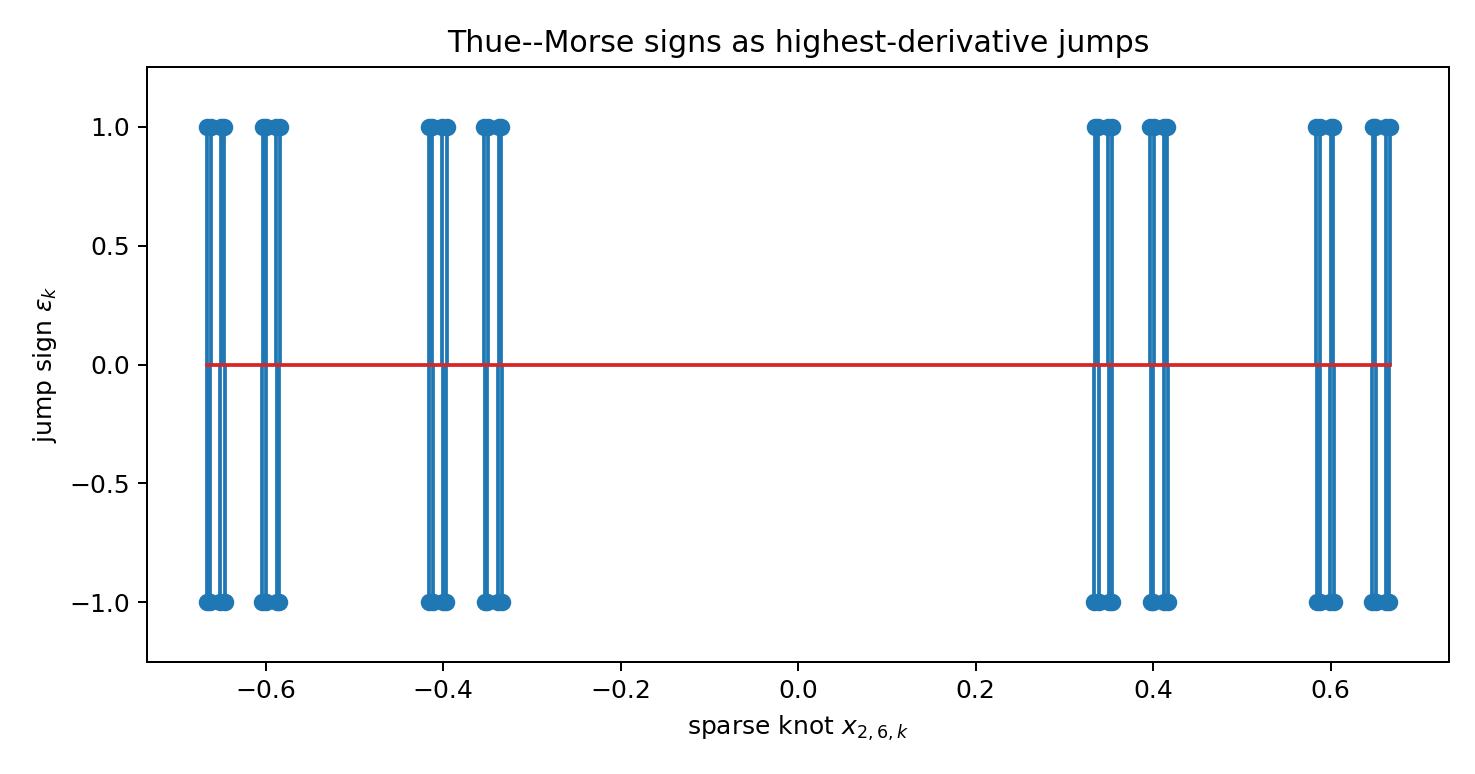
\includegraphics[width=0.94\textwidth]{thue_morse_jump_comb.png}
\caption{The distribution $q^{\binom N2}D^Ng_{r,N}$ for a finite sparse
spline.  Reading its signed atoms from left to right gives the ordinary
Thue--Morse word because the spatial bit-reversal leaves binary parity
unchanged.  The plotted example is generated by the accompanying script.}
\label{fig:TM-jump-comb}
\end{figure}

\begin{resultbox}[Contribution IV: Thue--Morse as analytic singular data]
The signed and unsigned Thue--Morse sequences can be recovered pointwise from
jumps of the highest classical derivative of a positive compact spline,
measure-theoretically from its next distributional derivative, integrally by
testing that derivative against cardinal functions, and spectrally from a
quotient of two sparse infinite sinc products.  In spatial order no external
binary labels are needed: the jumps already occur in Thue--Morse order.
\end{resultbox}

\section{Bell--Bernoulli power sums on sparse knots}
\label{sec:power-sums}

The jump measure immediately converts the moments of a positive box spline
into high-degree signed power sums.  This extends ordinary Prouhet cancellation
past its first nonzero degree and gives every surviving sum in closed Bell form.

\subsection{Prouhet cancellation and all surviving powers}

Let
\begin{equation}
 S_{r,N}(d)=\sum_{k=0}^{2^N-1}\eps_k x_{r,N,k}^{d}.         \label{eq:S-rNd}
\end{equation}

\begin{theorem}[Moment--power-sum duality]
\label{thm:moment-power-duality}
For $0\le d<N$,
\begin{equation}
 S_{r,N}(d)=0.                                             \label{eq:Prouhet-sparse}
\end{equation}
For every $m\ge0$,
\begin{equation}
 \boxed{\displaystyle
 S_{r,N}(N+m)=(-1)^Nq^{\binom N2}
   \frac{(N+m)!}{m!}\,\mu_m^{(r,N)},}                     \label{eq:power-sum-moment}
\end{equation}
where
\begin{equation}
 \mu_m^{(r,N)}=\int_{\R}x^m g_{r,N}(x)\,\dd x.            \label{eq:finite-moment}
\end{equation}
Equivalently,
\begin{equation}
 \boxed{\displaystyle
 \mu_m^{(r,N)}=(-1)^Nq^{-\binom N2}\frac{m!}{(N+m)!}
   \sum_{k<2^N}\eps_kx_{r,N,k}^{N+m}.}                   \label{eq:moment-from-TM}
\end{equation}
Odd $m$ give zero by symmetry.
\end{theorem}

\begin{proof}
Pair \eqref{eq:DNg-comb} with the polynomial $x^d$.  If $d<N$, its $N$th
derivative vanishes.  If $d=N+m$, distributional integration by parts gives
\[
 q^{-\binom N2}S_{r,N}(N+m)
 =(-1)^N\frac{(N+m)!}{m!}\int x^m g_{r,N}(x)\,\dd x.
\]
Rearrange.
\end{proof}

The first two nontrivial cases are
\begin{align}
 \sum_{k<2^N}\eps_kx_{r,N,k}^{N}
 &=(-1)^NN!q^{\binom N2},                                 \label{eq:first-survivor}\\
 \sum_{k<2^N}\eps_kx_{r,N,k}^{N+2}
 &=(-1)^Nq^{\binom N2}\frac{(N+2)!}{24}
   \frac{1-q^{2N}}{1-q^2}.                                \label{eq:second-survivor}
\end{align}
Thus the full hierarchy refines the usual statement that the first surviving
Prouhet power occurs in degree $N$.

\subsection{Finite cumulants and complete Bell form}

The moment-generating function of $Z_{r,N}$ is
\begin{equation}
 M_{r,N}(s)=\prod_{j=0}^{N-1}\frac{\sinh(sq^j/2)}{sq^j/2}. \label{eq:MrN}
\end{equation}
Its cumulants are finite geometric truncations of the sparse cumulants.

\begin{proposition}[Finite sparse cumulants]
\label{prop:finite-sparse-cumulants}
For $\ell\ge1$,
\begin{equation}
 \kappa_{2\ell}^{(r,N)}
 =\frac{B_{2\ell}}{2\ell}
   \frac{1-q^{2\ell N}}{1-q^{2\ell}},
 \qquad
 \kappa_{2\ell+1}^{(r,N)}=0.                              \label{eq:finite-cumulants}
\end{equation}
Hence
\begin{equation}
 \mu_m^{(r,N)}
 =\cB_m\bigl(0,\kappa_2^{(r,N)},0,\kappa_4^{(r,N)},\ldots\bigr). \label{eq:finite-Bell-moments}
\end{equation}
Combining with \eqref{eq:power-sum-moment} gives an explicit
Bell--Bernoulli formula for every signed power sum $S_{r,N}(N+m)$.
\end{proposition}

In particular, for $\ell\ge0$,
\begin{equation}
 S_{r,N}(N+2\ell)
 =(-1)^Nq^{\binom N2}\frac{(N+2\ell)!}{(2\ell)!}
 \cB_{2\ell}\bigl(0,\kappa_2^{(r,N)},0,\ldots,
                    \kappa_{2\ell}^{(r,N)}\bigr).          \label{eq:Bell-power-sum}
\end{equation}
This is a finite product--series--Bell representation in which every parameter
is rational for $q=2^{-r}$.

\subsection{Unsigned power sums}

The total knot comb $\Lambda_{r,N}$ is the unnormalized law of the centered
Bernoulli sum
\begin{equation}
 W_{r,N}=\sum_{j=0}^{N-1}q^j(B_j-\tfrac12),
 \qquad \Prob(B_j=0)=\Prob(B_j=1)=\tfrac12.                \label{eq:W-rN}
\end{equation}
Its even cumulants are
\begin{equation}
 \lambda_{2\ell}^{(r,N)}
 =\frac{(2^{2\ell}-1)B_{2\ell}}{2\ell}
   \frac{1-q^{2\ell N}}{1-q^{2\ell}},                    \label{eq:Bernoulli-knot-cumulants}
\end{equation}
with odd cumulants zero.  Therefore
\begin{equation}
 T_{r,N}(d):=\sum_{k<2^N}x_{r,N,k}^d
 =2^N\cB_d(0,\lambda_2^{(r,N)},0,\lambda_4^{(r,N)},\ldots). \label{eq:total-knot-power}
\end{equation}
If
\begin{align}
 T_{r,N}^{\mathrm{evil}}(d)&=\sum_{\tau(k)=0}x_{r,N,k}^d, \\
 T_{r,N}^{\mathrm{odious}}(d)&=\sum_{\tau(k)=1}x_{r,N,k}^d,
\end{align}
then
\begin{align}
 T_{r,N}^{\mathrm{evil}}(d)
 &=\frac{T_{r,N}(d)+S_{r,N}(d)}2,                          \label{eq:evil-power}\\
 T_{r,N}^{\mathrm{odious}}(d)
 &=\frac{T_{r,N}(d)-S_{r,N}(d)}2.                          \label{eq:odious-power}
\end{align}
For $d<N$ the two values coincide; for $d=N+m$ their exact difference is
\eqref{eq:power-sum-moment}.  Thus the unsigned partition inherits a complete
Bell--Bernoulli moment calculus, not only the usual equality up to degree
$N-1$.

\subsection{Infinite moment limits}

Since $Z_{r,N}\to Z_r$ almost surely and uniformly in the underlying cube,
all moments converge.  Therefore \eqref{eq:moment-from-TM} gives
\begin{equation}
 \boxed{\displaystyle
 \mu_m^{(r)}
 =\lim_{N\to\infty}(-1)^Nq^{-\binom N2}\frac{m!}{(N+m)!}
 \sum_{k<2^N}\eps_kx_{r,N,k}^{N+m}.}                     \label{eq:sparse-moment-TM-limit}
\end{equation}
At $r=1$, these are the moments of Rvachev's up-function:
\begin{equation}
 \int_{-1}^{1}x^m u(x)\,\dd x
 =\lim_{N\to\infty}(-1)^N2^{\binom N2}\frac{m!}{(N+m)!}
 \sum_{k<2^N}\eps_kx_{1,N,k}^{N+m}.                      \label{eq:up-moment-TM-limit}
\end{equation}
The enormous factor $q^{-\binom N2}$ exactly renormalizes the Prouhet
cancellation.

Moments of the bounded Fabius law and powers of the inverse follow from
$Y=(X+1)/2$:
\begin{align}
 \int_0^1G(y)^m\,\dd y
 &=\E Y^m
 =2^{-m}\sum_{j=0}^m\binom mj\mu_j,                       \label{eq:G-moment-up}\\
 \int_0^1x^pF(x)\,\dd x
 &=\frac{1-\E Y^{p+1}}{p+1},\qquad \Re p>-1.              \label{eq:F-Mellin-moment}
\end{align}
Substitution of \eqref{eq:up-moment-TM-limit} therefore yields explicit
Thue--Morse limit representations for both integrals.

\subsection{A Gaussian \texorpdfstring{$q$}{q}-binomial side identity}

The same binary digits carry a second geometric statistic
$\sigma(k)=\sum_jjb_j(k)$.  Its joint Hamming-weight enumerator is
\begin{equation}
 \sum_{k<2^N}y^{s_2(k)}q^{\sigma(k)}
 =\prod_{j=0}^{N-1}(1+yq^j)
 =\sum_{h=0}^{N}y^hq^{\binom h2}\qbinom Nhq.               \label{eq:qbinomial-digit-enumerator}
\end{equation}
This familiar Gaussian-binomial identity is not the same as the knot transform
\eqref{eq:master-knot-enumerator}: one weights a selected digit by $q^j$, the
other places it at the geometric coordinate $q^j$.  Their coexistence is useful
in symbolic calculations because the first organizes selected scale indices,
while the second organizes the actual spline knots.

\begin{resultbox}[Contribution V: all Prouhet survivors]
The finite sparse spline does more than explain cancellation below degree $N$.
Its moments give every surviving signed power sum in degree $N+m$, and finite
uniform cumulants turn the answer into a closed Bell polynomial in Bernoulli
numbers and geometric factors.  Adding the cosh-product moments of the unsigned
knot comb gives separate exact formulas for the evil and odious classes.
\end{resultbox}

\section{Infinite products of averaging operators}
\label{sec:operators}

The Fourier product can be read literally as a product of physical-space
averaging operators.  This provides a representation which is simultaneously
probabilistic, convolutional, and an infinite-order differential calculus.

\subsection{Uniform averaging and strong product limits}

For $a>0$, define
\begin{equation}
 (\cU_af)(x)=\frac1{2a}\int_{-a}^{a}f(x-t)\,\dd t.         \label{eq:Ua-def}
\end{equation}
Its Fourier multiplier and formal differential symbol are
\begin{equation}
 \widehat{\cU_af}(z)=\sincpi(2az)\widehat f(z),
 \qquad
 \cU_a=\frac{\sinh(aD)}{aD}.                              \label{eq:Ua-symbol}
\end{equation}
The second equality is exact on polynomials and on every class on which the
translation exponential may be integrated termwise.

Put
\begin{equation}
 \cG_{r,N}=\prod_{j=0}^{N-1}\cU_{q^j/2},
 \qquad
 \cG_r=\prod_{j=0}^{\infty}\cU_{q^j/2}.                  \label{eq:Gr-operator}
\end{equation}
The factors commute.

\begin{theorem}[Averaging-operator representation]
\label{thm:averaging-operator}
For every bounded uniformly continuous $f$,
\begin{align}
 (\cG_{r,N}f)(x)&=(g_{r,N}*f)(x)=\E f(x-Z_{r,N}),          \label{eq:GrN-convolution}\\
 (\cG_rf)(x)&=(g_r*f)(x)=\E f(x-Z_r),                     \label{eq:Gr-convolution}
\end{align}
and $\cG_{r,N}f\to\cG_rf$ uniformly.  The same convergence is strong on
$L^p(\R)$ for $1\le p<\infty$.  Distributionally,
\begin{equation}
 g_{r,N}=\cG_{r,N}\delta_0,
 \qquad
 g_r=\cG_r\delta_0.                                       \label{eq:g-operator-delta}
\end{equation}
For $r=1$ this gives
\begin{equation}
 u=\left(\prod_{j=0}^{\infty}\cU_{2^{-j-1}}\right)\delta_0. \label{eq:u-averaging-product}
\end{equation}
\end{theorem}

\begin{proof}
Each operator convolves with the density of a centered uniform random variable
of half-width $q^j/2$.  Finite products therefore give the law of $Z_{r,N}$.
The tail satisfies $|Z_r-Z_{r,N}|\le A_rq^N$ pointwise on the underlying
product space, which proves uniform convergence for uniformly continuous $f$.
Strong $L^p$ convergence follows from continuity of translations in $L^p$ and
dominated averaging.  Applying the convolution operators to $\delta_0$ gives
the densities.
\end{proof}

\subsection{Bernoulli logarithm of the operator product}

The classical expansion
\begin{equation}
 \log\frac{\sinh z}{z}
 =\sum_{m=1}^{\infty}
   \frac{2^{2m-1}B_{2m}}{m(2m)!}z^{2m}                   \label{eq:log-sinh}
\end{equation}
shows that the logarithm of the sparse averaging product is controlled by the
same Bernoulli cumulants as the random law.

Define
\begin{equation}
 c_{r,m}=\frac{B_{2m}}{2m(2m)!(1-q^{2m})}.                 \label{eq:crm}
\end{equation}

\begin{theorem}[Infinite-order differential representation]
\label{thm:infinite-differential-operator}
As a formal differential operator, and exactly on every polynomial,
\begin{align}
 \boxed{\displaystyle
 \cG_r
 =\exp\!\left(\sum_{m=1}^{\infty}c_{r,m}D^{2m}\right),}  \label{eq:Gr-exponential}\\
 \cG_{r,N}
 &=\exp\!\left(\sum_{m=1}^{\infty}
       c_{r,m}(1-q^{2mN})D^{2m}\right).                   \label{eq:GrN-exponential}
\end{align}
If $f$ has Fourier support in a compact subset of $(-1,1)$, then
\eqref{eq:Gr-exponential} is also an exact Fourier-multiplier identity.
For the classical up-function,
\begin{equation}
 \boxed{\displaystyle
 u=\exp\!\left(
   \frac{D^2}{18}-\frac{D^4}{2700}+\frac{D^6}{178605}
   -\frac{D^8}{9639000}+\cdots\right)\delta_0,}           \label{eq:u-differential-exponential}
\end{equation}
where the equality is understood through the exact averaging product and,
termwise, through its formal or band-limited expansion.
\end{theorem}

\begin{proof}
From \eqref{eq:Ua-symbol} and \eqref{eq:log-sinh},
\[
 \log\cU_{q^j/2}
 =\sum_{m\ge1}\frac{B_{2m}}{2m(2m)!}q^{2mj}D^{2m}.
\]
Summing over $j$ gives \eqref{eq:Gr-exponential}; truncating the geometric sum
gives \eqref{eq:GrN-exponential}.  On a polynomial only finitely many
powers of $D$ survive.  On Fourier support $|z|<1$, substitution
$D\mapsto2\pi\ii z$ gives precisely the convergent series
\eqref{eq:Psi-log-zeta}.  The displayed coefficients in
\eqref{eq:u-differential-exponential} are $c_{1,m}$.
\end{proof}

Using Euler's formula for $\zeta(2m)$, the same operator can be written
\begin{equation}
 \cG_r
 =\exp\!\left(
   \sum_{m=1}^{\infty}
   \frac{(-1)^{m+1}\zeta(2m)}{m(1-q^{2m})(2\pi)^{2m}}
   D^{2m}\right).                                        \label{eq:Gr-zeta-operator}
\end{equation}
Thus the Bernoulli, zeta, cumulant, and Fourier-logarithm representations are
literally the same coefficients in four coordinate systems.

\subsection{Exact tail operators and series--product combinations}

Let $\cT_{r,N}$ be convolution by the scaled tail density
$q^{-N}g_r(\cdot/q^N)$.  Then
\begin{equation}
 \cG_r=\cT_{r,N}\cG_{r,N},
 \qquad
 \widehat{\cT_{r,N}f}(z)=\Psi_r(q^Nz)\widehat f(z).       \label{eq:tail-operator-factor}
\end{equation}
On polynomials and in the low-frequency calculus,
\begin{equation}
 \cT_{r,N}
 =\exp\!\left(\sum_{m=1}^{\infty}c_{r,m}q^{2mN}D^{2m}\right). \label{eq:tail-exponential}
\end{equation}
Consequently, for every polynomial $p$,
\begin{equation}
 \int p(x-y)g_r(y)\,\dd y
 =\exp\!\left(\sum_{m\ge1}c_{r,m}D^{2m}\right)p(x),       \label{eq:polynomial-exact-operator}
\end{equation}
and
\begin{equation}
 \int p(x-y)q^{-N}g_r(y/q^N)\,\dd y
 =\exp\!\left(\sum_{m\ge1}c_{r,m}q^{2mN}D^{2m}\right)p(x). \label{eq:tail-polynomial-operator}
\end{equation}
Expanding the last exponential gives the exact finite identity
\begin{equation}
 \E p(x-q^NZ_r)
 =\sum_{m=0}^{\deg p}\frac{(-q^N)^m\mu_m^{(r)}}{m!}p^{(m)}(x), \label{eq:tail-Taylor-polynomial}
\end{equation}
whose odd terms vanish.  This is a rigorous series--integral representation,
not an asymptotic expansion, whenever the test function is a polynomial.

For analytic or smooth functions the same coefficients organize the familiar
small-tail expansion.  The first two even orders are
\begin{equation}
 \cT_{r,N}
 =I+c_{r,1}q^{2N}D^2+
   \left(c_{r,2}+\frac{c_{r,1}^2}{2}\right)q^{4N}D^4
   +\bigO_{\mathrm{formal}}(q^{6N}D^6).                   \label{eq:tail-first-orders}
\end{equation}
The coefficient of $q^{2mN}D^{2m}$ is equivalently
$\mu_{2m}^{(r)}/(2m)!$, by the Bell relation between cumulants and moments.

\subsection{Reciprocal and deconvolution operators}

Since $\widehat{g_{r,N}}=\Psi_r/\Psi_r(q^N\cdot)$, the finite spline is a
formal deconvolution of the smooth limit:
\begin{equation}
 g_{r,N}
 =\exp\!\left(-\sum_{m\ge1}c_{r,m}q^{2mN}D^{2m}\right)g_r. \label{eq:formal-deconvolution}
\end{equation}
This identity is exact as a germ of Fourier multipliers at the origin and gives
all algebraic orders in $q^{2N}$.  Its global use requires the zero-aware
factorization \eqref{eq:g-rN-Fourier}, because the reciprocal of
$\Psi_r(q^Nz)$ has poles which are cancelled by zeros of $\Psi_r(z)$.
That distinction is important: the product quotient is globally exact, while
the exponential reciprocal is a local or asymptotic coordinate chart.

The first logarithmic coefficients, generated exactly by the accompanying
script, are shown in \cref{tab:operator-coefficients}.

\begin{table}[htbp]
\centering
\small
\begin{tabular}{@{}c c c c@{}}
\toprule
$2m$ & $c_{1,m}$ & $c_{2,m}$ & $c_{3,m}$\\
\midrule
2 & $1/18$ & $2/45$ & $8/189$\\
4 & $-1/2700$ & $-4/11475$ & $-64/184275$\\
6 & $1/178605$ & $64/11609325$ & $4096/743175405$\\
8 & $-1/9639000$ & $-32/309652875$ & $-8192/79272340875$\\
10 & $1/478533825$ & $1024/490497170625$ & $1048576/502269581253825$\\
\bottomrule
\end{tabular}
\caption{Coefficients of $D^{2m}$ in $\log\cG_r$.  The complete exact table
through order $16$ is included as \texttt{operator\_coefficients.csv}.}
\label{tab:operator-coefficients}
\end{table}

\begin{resultbox}[Contribution VI: an operator logarithm]
The infinite sinc product is the Fourier symbol of an infinite product of
uniform averaging operators.  Its logarithm is an even differential operator
whose coefficients are simultaneously sparse cumulants, Bernoulli numbers,
and zeta values.  On polynomials the exponential representation is exact; on
band-limited functions it is an exact multiplier; globally the averaging
product supplies the canonical interpretation.
\end{resultbox}

\section{Twisted Poisson and zero-slope representations}
\label{sec:Zak}

The critical half-integer cosine series is one member of a continuous family
obtained by twisting Poisson summation.  This family also yields a representation
of $F$ through the derivatives of $\Phi$ at its integer zeros.

\subsection{A one-parameter Zak family}

For real $\alpha$, define
\begin{equation}
 Z_u(x,\alpha)=\sum_{n\in\Z}u(x+n)\e^{-2\pi\ii n\alpha}.   \label{eq:Zak-def}
\end{equation}
Rapid decay of $\Phi$ and compact support of $u$ justify Poisson summation
absolutely in the forms used below.

\begin{theorem}[Twisted spectral representation of $F$]
\label{thm:twisted-F}
For $0\le x\le1$,
\begin{equation}
 Z_u(x,\alpha)
 =\sum_{k\in\Z}\Phi(k+\alpha)
   \e^{2\pi\ii(k+\alpha)x}                                \label{eq:Zak-Poisson}
\end{equation}
and also
\begin{equation}
 Z_u(x,\alpha)=1+(\e^{2\pi\ii\alpha}-1)F(x).             \label{eq:Zak-fold}
\end{equation}
Hence, whenever $\alpha\notin\Z$,
\begin{equation}
 \boxed{\displaystyle
 F(x)=\frac{
   \sum_{k\in\Z}\Phi(k+\alpha)
       \e^{2\pi\ii(k+\alpha)x}-1}
  {\e^{2\pi\ii\alpha}-1}.}                              \label{eq:F-twisted-Poisson}
\end{equation}
Using polyphase factors, each coefficient may be replaced by
$\prod_{a=0}^{r-1}\Psi_r((k+\alpha)/2^a)$.
\end{theorem}

\begin{proof}
The modulated Poisson formula gives \eqref{eq:Zak-Poisson}.  On the interval
$0<x<1$, only the translates $n=0$ and $n=-1$ meet the support of $u$, so
\[
 Z_u(x,\alpha)=u(x)+\e^{2\pi\ii\alpha}u(x-1)
 =1-F(x)+\e^{2\pi\ii\alpha}F(x).
\]
Continuity supplies the endpoint values.
\end{proof}

At $\alpha=1/2$, \eqref{eq:F-twisted-Poisson} becomes the real cosine series
\begin{equation}
 F(x)=\frac12-
 \sum_{k=0}^{\infty}\Phi(k+\tfrac12)
   \cos((2k+1)\pi x),                                     \label{eq:F-half-integer-cosine}
\end{equation}
which is the shifted form of \eqref{eq:critical-cosine}.  Rational values of
$\alpha$ give cyclotomic spectral expansions; irrational values give a
continuous family of quasiperiodic representations.

\subsection{Differentiating through the untwisted limit}

Both numerator and denominator of \eqref{eq:F-twisted-Poisson} vanish at
$\alpha=0$.  Differentiation gives a new zero-jet representation.

\begin{corollary}[Integer-zero slope series]
\label{cor:zero-slope-F}
For $0\le x\le1$,
\begin{align}
 F(x)
 &=x+\frac1{2\pi\ii}
   \sum_{k\in\Z\setminus\{0\}}\Phi'(k)\e^{2\pi\ii kx}    \label{eq:F-zero-slope-complex}\\
 &=x+\frac1\pi\sum_{k=1}^{\infty}\Phi'(k)
   \sin(2\pi kx)                                         \label{eq:F-zero-slope-real}\\
 &=x-\frac1\pi\sum_{m=0}^{\infty}
   \frac{\Phi(m+\tfrac12)}{2m+1}
   \sin(2\pi(2m+1)x).                                    \label{eq:F-half-slope-series}
\end{align}
Only odd positive integers contribute in the middle series.
\end{corollary}

\begin{proof}
Differentiate \eqref{eq:Zak-Poisson} at $\alpha=0$ and use
\eqref{eq:Zak-fold}.  Since $\Phi(0)=1$, $\Phi'(0)=0$, and
$\Phi(k)=0$ for nonzero integers, division by $2\pi\ii$ gives
\eqref{eq:F-zero-slope-complex}.  Pair $k$ with $-k$ to obtain the real sine
series.  If $k$ is even, the zero has order at least two, so $\Phi'(k)=0$.
For odd $k=2m+1$, the first sinc factor has a simple zero and
\begin{equation}
 \Phi'(2m+1)=-\frac{\Phi(m+\tfrac12)}{2m+1},               \label{eq:odd-zero-slope}
\end{equation}
which gives \eqref{eq:F-half-slope-series}.
\end{proof}

The transform formula \eqref{eq:F-Fourier} also yields, for real $\xi\ne0$,
\begin{align}
 \int_0^1F(x)\cos(2\pi\xi x)\,\dd x
 &=\frac{\sin(2\pi\xi)-\Phi(\xi/2)\sin(\pi\xi)}{2\pi\xi}, \label{eq:F-cos-transform}\\
 \int_0^1F(x)\sin(2\pi\xi x)\,\dd x
 &=\frac{\Phi(\xi/2)\cos(\pi\xi)-\cos(2\pi\xi)}{2\pi\xi}. \label{eq:F-sin-transform}
\end{align}
At integer frequencies the cosine coefficients vanish, while the sine
coefficients are explicit samples of $\Phi$.

\begin{resultbox}[Contribution VII: a continuous spectral family]
The usual half-integer cosine expansion sits inside a twisted Poisson family
parameterized by $\alpha$.  Letting the twist tend to zero converts spectral
values into spectral slopes and yields a sine series for $F$ supported exactly
on the simple odd zeros of the Rvachev Fourier product.
\end{resultbox}

\section{Sparse lobe signs and base-\texorpdfstring{$2^r$}{2-to-the-r} digit sums}
\label{sec:sparse-signs}

The staircase zero multiplicities of $\Psi_r$ generate a natural automatic
sign sequence.  Polyphase recombination then factors the ordinary Thue--Morse
sign into $r$ such sparse signs.

Let $s_b(n)$ denote the sum of the base-$b$ digits of $n$.

\begin{theorem}[Lobe signs of a sparse sinc product]
\label{thm:sparse-lobe-sign}
For $n\ge0$ and any $x\in(n,n+1)$,
\begin{align}
 \sgn\Psi_r(x)
 &=(-1)^{\sum_{j=1}^{n}m_r(j)}                             \label{eq:sparse-sign-zero-count}\\
 &=(-1)^{n+\sum_{\ell\ge1}\lfloor n/2^{r\ell}\rfloor}    \label{eq:sparse-sign-floor}\\
 &=\boxed{(-1)^{s_{2^r}(n)}}.                             \label{eq:sparse-sign-base}
\end{align}
Thus the signs of the consecutive real lobes of $\Psi_r$ form the parity-of-
digit-sum sequence in base $2^r$.
\end{theorem}

\begin{proof}
The sign starts positive on $(0,1)$ and flips once for each zero multiplicity
crossed, giving \eqref{eq:sparse-sign-zero-count}.  Since
$m_r(j)=1+\lfloor\nu_2(j)/r\rfloor$,
\[
 \sum_{j=1}^{n}\left\lfloor\frac{\nu_2(j)}r\right\rfloor
 =\sum_{\ell\ge1}\#\{j\le n:2^{r\ell}\mid j\}
 =\sum_{\ell\ge1}\left\lfloor\frac n{2^{r\ell}}\right\rfloor.
\]
For $b=2^r$, the base-$b$ Legendre identity is
\[
 \sum_{\ell\ge1}\left\lfloor\frac n{b^\ell}\right\rfloor
 =\frac{n-s_b(n)}{b-1}.
\]
Because $b-1$ is odd and $b$ is even,
$n+(n-s_b(n))/(b-1)$ has the same parity as $s_b(n)$.
\end{proof}

At $r=1$, \eqref{eq:sparse-sign-base} is the familiar formula
$\sgn\Phi(x)=\eps_n$ on the $n$th lobe.  For $r>1$ it supplies a companion
automatic sequence attached to the sparse Rvachev density.

\begin{corollary}[Polyphase factorization of the Thue--Morse sign]
\label{cor:TM-base-factorization}
For every $r\ge1$ and $n\ge0$,
\begin{equation}
 \boxed{\displaystyle
 \eps_n
 =\prod_{a=0}^{r-1}(-1)^{s_{2^r}(\lfloor n/2^a\rfloor)}.} \label{eq:TM-base-factorization}
\end{equation}
Equivalently,
\begin{equation}
 \boxed{\displaystyle
 \tau(n)\equiv
 \sum_{a=0}^{r-1}s_{2^r}(\lfloor n/2^a\rfloor)\pmod2.}   \label{eq:TM-base-parity}
\end{equation}
The same representation is analytic:
\begin{equation}
 \eps_n
 =\prod_{a=0}^{r-1}
   \sgn\Psi_r\!\left(\frac{n+1/2}{2^a}\right).           \label{eq:TM-sparse-lobe-product}
\end{equation}
\end{corollary}

\begin{proof}
Take signs in the polyphase product
$\Phi(n+1/2)=\prod_a\Psi_r((n+1/2)/2^a)$.  The argument of the $a$th factor
lies in the lobe indexed by $\lfloor n/2^a\rfloor$.  Apply
\cref{thm:sparse-lobe-sign} and use
$\sgn\Phi(n+1/2)=\eps_n$.  The unsigned parity form is the exponent modulo two.
\end{proof}

An entirely arithmetical proof follows by summing the floor exponents:
\begin{equation}
 \sum_{a=0}^{r-1}\sum_{m\ge0}
 \left\lfloor\frac{n}{2^{a+rm}}\right\rfloor
 =\sum_{j\ge0}\left\lfloor\frac{n}{2^j}\right\rfloor
 =2n-s_2(n),                                               \label{eq:floor-polyphase-TM}
\end{equation}
whose parity is $s_2(n)$.  Formula
\eqref{eq:TM-base-factorization} therefore expresses binary digit parity as a
cyclic product of overlapping base-$2^r$ digit parities.

\begin{corollary}[Thue--Morse from odd zero slopes]
\label{cor:TM-zero-slopes}
For every $n\ge0$,
\begin{equation}
 \boxed{\displaystyle
 \eps_n=-\sgn\Phi'(2n+1),
 \qquad
 \tau(n)=\frac{1+\sgn\Phi'(2n+1)}2.}                      \label{eq:TM-zero-slope-sign}
\end{equation}
\end{corollary}

\begin{proof}
Equation \eqref{eq:odd-zero-slope} says
$\Phi'(2n+1)=-\Phi(n+1/2)/(2n+1)$.  The lobe sign of the half-integer value is
$\eps_n$.
\end{proof}

\begin{resultbox}[Contribution VIII: a new digital factorization]
The sparse component does not merely split amplitudes.  Its lobe signs are
base-$2^r$ digit-parity characters, and their $r$ shifted polyphase copies
multiply to the binary Thue--Morse character.  This gives both a new purely
digital formula and a product of analytic sign samples.  Odd zero slopes of the
full Fourier image give a second pointwise analytic representation.
\end{resultbox}

\section{Representation concordance}
\label{sec:concordance}

This section gathers the formulas into a compact lookup index.  A reader
interested in a particular mode---probability, transform, product, series,
operator, geometry, or combinatorics---can use the rightmost column to locate
the hypotheses and proof.  The list includes both corpus baseline and the new
polyphase layer; it is not a novelty list.

\subsection{Rvachev's up-function and its Fourier image}

\renewcommand{\arraystretch}{1.22}
\begin{longtable}{@{}p{0.18\textwidth}p{0.69\textwidth}p{0.07\textwidth}@{}}
\toprule
Viewpoint & Representation & Status\\
\midrule
\endfirsthead
\toprule
Viewpoint & Representation & Status\\
\midrule
\endhead
Random series &
$X=\sum_{n\ge0}2^{-n-1}U_n$, with $u$ the density of $X$. & \statusknown\\
Infinite cube &
$u(x)=\int_{[-1,1]^{\N}}\delta(x-\sum2^{-n-1}v_n)\prod\dd v_n/2$ in the distributional sense. & \statusknown\\
Finite convolution &
$u=\lim_{N\to\infty}g_{1,N}$, where $g_{1,N}$ is an explicit nonuniform box spline. & \statusknown\\
Self-CDF &
$u(x)=\Prob(X\le2x+1)$ for $-1\le x\le0$, equivalently $u(x)=F(x+1)$. & \statusknown\\
Delay equation &
$u'(x)=2(u(2x+1)-u(2x-1))$. & \statusknown\\
Derivative cascade &
$u^{(N)}(x)=2^{N(N+1)/2}\sum_{k<2^N}\eps_k
u(2^Nx+2^N-1-2k)$. & \statusknown\\
Fourier inversion &
$u(x)=\int_{\R}\Phi(z)\e^{2\pi\ii zx}\dd z
=2\int_0^\infty\Phi(z)\cos(2\pi zx)\dd z$. & \statusknown\\
Characteristic expectation &
$\Phi(z)=\E\e^{-2\pi\ii zX}$. & \statusknown\\
Sinc product &
$\Phi(z)=\prod_{n\ge0}\sincpi(z/2^n)$. & \statusknown\\
Triangular cosine product &
$\Phi(z)=\prod_{m\ge1}\cos(\pi z/2^m)^m$. & \statusknown\\
Canonical zero product &
$\Phi(z)=\prod_{n\ge1}(1-z^2/n^2)^{1+\nu_2(n)}$. & \statusknown\\
Gamma product &
$\Phi(z)=\prod_{n\ge0}[\Gamma(1+z/2^n)\Gamma(1-z/2^n)]^{-1}$. & \statusknown\\
Logarithmic zeta series &
$\log\Phi(z)=-\sum_{m\ge1}\zeta(2m)z^{2m}/[m(1-4^{-m})]$, $|z|<1$. & \statusknown\\
Cotangent logarithmic derivative &
$\Phi'/\Phi=\sum_{j\ge0}[(\pi/2^j)\cot(\pi z/2^j)-1/z]$. & \statusderived\\
Tangent logarithmic derivative &
$\Phi'/\Phi=-\pi\sum_{m\ge1}m2^{-m}\tan(\pi z/2^m)$. & \statusderived\\
Partial fractions &
$\Phi'/\Phi=-2z\sum_{n\ge1}(1+\nu_2(n))/(n^2-z^2)$. & \statusknown\\
Moment-generating product &
$M(s)=\prod_{n\ge0}\sinh(s/2^{n+1})/(s/2^{n+1})$. & \statusknown\\
Moment series &
$M(s)=\sum_{m\ge0}\mu_ms^m/m!$, with
$\mu_m=\cB_m(\kappa_1,\ldots,\kappa_m)$. & \statusknown\\
Cumulants &
$\kappa_{2m}=B_{2m}/[2m(1-4^{-m})]$, $\kappa_{2m+1}=0$. & \statusknown\\
Critical cosine series &
$u(x)=\tfrac12+\sum_{k\ge0}\Phi(k+\tfrac12)\cos((2k+1)\pi x)$. & \statusknown\\
Partition of unity &
$\sum_{j\in\Z}u(x-j)=1$. & \statusknown\\
Twisted Zak transform &
$\sum_nu(x+n)\e^{-2\pi\ii n\alpha}
=\sum_k\Phi(k+\alpha)\e^{2\pi\ii(k+\alpha)x}$. & \statusderived\\
Legendre expansion &
$u(x)=\sum_{n\ge0}a_{2n}P_{2n}(x)$,
$a_{2n}=\frac{4n+1}{2}\int_{-1}^{1}u(x)P_{2n}(x)\dd x$;
all coefficients reduce to moments. & \statusknown\\
Haar, Walsh, and Schauder &
Exact rational multiresolution expansions and finite Walsh products are developed in \cite{repoMultiresolution}. & \statusknown\\
Cauchy transform &
$R(z)=\int u(x)/(z-x)\dd x=\sum_{m\ge0}\mu_mz^{-m-1}$. & \statusknown\\
Jacobi fraction &
$R(z)=1/(z-a_0-b_1/(z-a_1-b_2/(\cdots)))$, with coefficients determined by the moment Hankel determinants. & \statusknown\\
Fredholm determinant &
$\Phi(z)=\det(I-z^2T)$ for eigenvalues $n^{-2}$ of multiplicity $1+\nu_2(n)$. & \statusknown\\
Spectral zeta &
$\sum_{n\ge1}(1+\nu_2(n))n^{-s}=\zeta(s)/(1-2^{-s})$. & \statusknown\\
Heat trace &
$K(t)=\sum_{n\ge1}(1+\nu_2(n))\e^{-tn^2}$ and
$\int_0^\infty t^{s/2-1}K(t)\dd t=\Gamma(s/2)\zeta(s)/(1-2^{-s})$. & \statusderived\\
Polyphase product &
$\Phi(z)=\prod_{a=0}^{r-1}\Psi_r(z/2^a)$. & \statusnew\\
Polyphase convolution &
$u=*_{a=0}^{r-1}\bigl(2^ag_r(2^a\,\cdot)\bigr)$. & \statusnew\\
Radon section &
$u(t)=\norm{w_r}^{-1}\int_{w_r\cdot y=t}\prod_ag_r(y_a)\dd\sigma$. & \statusnew\\
Averaging product &
$u=(\prod_{j\ge0}\cU_{2^{-j-1}})\delta_0$. & \statusnew\\
Differential exponential &
$u=\exp(\sum_{m\ge1}B_{2m}D^{2m}/[2m(2m)!(1-4^{-m})])\delta_0$, interpreted as in \cref{sec:operators}. & \statusnew\\
\bottomrule
\end{longtable}

\subsection{The bounded and inverse Fabius functions}

\begin{longtable}{@{}p{0.18\textwidth}p{0.69\textwidth}p{0.07\textwidth}@{}}
\toprule
Viewpoint & Representation & Status\\
\midrule
\endfirsthead
\toprule
Viewpoint & Representation & Status\\
\midrule
\endhead
CDF &
$F(x)=\Prob(X\le2x-1)$. & \statusknown\\
Fold &
$F(x)=u(x-1)$ and $F(1-x)=u(x)$. & \statusknown\\
Symmetry &
$F(1-x)=1-F(x)$. & \statusknown\\
Differential equation &
$F'(x)=2F(2x)$ on $0\le x\le1/2$. & \statusknown\\
Density Fourier integral &
$F(x)=\int_{\R}\Phi(z)\e^{2\pi\ii z(x-1)}\dd z$. & \statusknown\\
CDF sine integral &
$F(x)=\tfrac12+\pi^{-1}\int_0^\infty\Phi(z)
\sin(2\pi z(2x-1))\dd z/z$. & \statusknown\\
Product integral &
Replace $\Phi$ in either preceding integral by its sinc, cosine, Gamma, canonical, or polyphase product. & \statusderived\\
Laplace--Stieltjes &
$\int_0^1\e^{sx}\dd F(x)=\e^{s/2}M(s/2)$. & \statusknown\\
Ordinary Laplace transform &
$\int_0^1\e^{sx}F(x)\dd x=(\e^s-\e^{s/2}M(s/2))/s$. & \statusknown\\
Bromwich inversion &
$F(x)=(2\pi\ii)^{-1}\int_{c-\ii\infty}^{c+\ii\infty}
\e^{s(x-1/2)}M(s/2)\dd s/s$. & \statusderived\\
Fourier image on $[0,1]$ &
$\widehat{F\mathbf1_{[0,1]}}(\xi)=
[\e^{-\pi\ii\xi}\Phi(\xi/2)-\e^{-2\pi\ii\xi}]/(2\pi\ii\xi)$. & \statusderived\\
Cosine transform &
Equation \eqref{eq:F-cos-transform}. & \statusderived\\
Sine transform &
Equation \eqref{eq:F-sin-transform}. & \statusderived\\
Half-integer cosine series &
$F(x)=\tfrac12-\sum_{k\ge0}\Phi(k+\tfrac12)\cos((2k+1)\pi x)$. & \statusknown\\
Twisted Poisson family &
Equation \eqref{eq:F-twisted-Poisson}, valid for every $\alpha\notin\Z$. & \statusnew\\
Zero-slope sine series &
$F(x)=x+\pi^{-1}\sum_{k\ge1}\Phi'(k)\sin(2\pi kx)$. & \statusnew\\
Half-integer slope series &
$F(x)=x-\pi^{-1}\sum_{m\ge0}\Phi(m+\tfrac12)
\sin(2\pi(2m+1)x)/(2m+1)$. & \statusnew\\
Moment integral &
$\int_0^1x^pF(x)\dd x=(1-\E Y^{p+1})/(p+1)$, $\Re p>-1$. & \statusknown\\
Polyphase volume &
$F(x)=\int_{w_r\cdot y\le2x-1}\prod_ag_r(y_a)\dd y$. & \statusnew\\
Polyphase section &
$F(x)=\norm{w_r}^{-1}\int_{w_r\cdot y=x-1}\prod_ag_r(y_a)\dd\sigma$. & \statusnew\\
Quantile level set &
$G(y)=\int_0^1\mathbf1_{\{F(x)\le y\}}\dd x$ for $0<y<1$. & \statusderived\\
Quantile transport &
$\int_0^1h(G(y))\dd y=\E h(Y)$. & \statusknown\\
Quantile moments &
$\int_0^1G(y)^m\dd y=\E Y^m$. & \statusknown\\
Quantile MGF &
$\int_0^1\e^{sG(y)}\dd y=\e^{s/2}M(s/2)$. & \statusknown\\
Inverse derivative &
$G'(y)=1/[2u(2G(y)-1)]$. & \statusknown\\
Radon quantile geometry &
$\cC_{w_r}p_r(2G(y)-1)=\cR_{w_r}p_r(G(y)-1)=y$. & \statusnew\\
Area duality &
$\int_0^1F(x)\dd x+\int_0^1G(y)\dd y=1$. & \statusknown\\
Dyadic arithmetic &
Finite Gaussian-$q$-binomial--Thue--Morse formulas for $F(m/2^n)$ are developed in \cite{repoPrimary,repoAtlas}. & \statusknown\\
Endpoint Lambert--$W$ &
The lower-branch Lambert coordinate and its periodic all-orders expansion are established in the audited asymptotic reports. & \statusknown\\
\bottomrule
\end{longtable}

\subsection{Signed and unsigned Thue--Morse representations}

\begin{longtable}{@{}p{0.19\textwidth}p{0.68\textwidth}p{0.07\textwidth}@{}}
\toprule
Viewpoint & Representation & Status\\
\midrule
\endfirsthead
\toprule
Viewpoint & Representation & Status\\
\midrule
\endhead
Binary definition &
$\eps_n=(-1)^{s_2(n)}$, $\tau(n)=(1-\eps_n)/2$. & \statusknown\\
Recursion &
$\eps_{2n}=\eps_n$, $\eps_{2n+1}=-\eps_n$; equivalently
$\tau(2n)=\tau(n)$, $\tau(2n+1)=1-\tau(n)$. & \statusknown\\
Floor-sum parity &
$\eps_n=(-1)^{n-\sum_{j\ge1}\lfloor n/2^j\rfloor}$. & \statusknown\\
Factorial valuation &
$\eps_n=(-1)^{n-\nu_2(n!)}$. & \statusknown\\
Finite coefficient product &
$\eps_n=[z^n]\prod_{j=0}^{N-1}(1-z^{2^j})$ for $n<2^N$. & \statusknown\\
Block Fourier product &
$\sum_{n<2^N}\eps_n\e^{2\pi\ii n\theta}
=\prod_{j<N}(1-\e^{2\pi\ii2^j\theta})$. & \statusknown\\
Prouhet moments &
$\sum_{n<2^N}\eps_nn^d=0$ for $d<N$. & \statusknown\\
Rvachev lobe sign &
$\eps_n=\sgn\Phi(n+\tfrac12)$. & \statusknown\\
Odd zero slope &
$\eps_n=-\sgn\Phi'(2n+1)$. & \statusnew\\
Sparse lobe product &
$\eps_n=\prod_{a=0}^{r-1}\sgn\Psi_r((n+1/2)/2^a)$. & \statusnew\\
Base-$2^r$ digit factorization &
$\eps_n=\prod_{a=0}^{r-1}(-1)^{s_{2^r}(\lfloor n/2^a\rfloor)}$. & \statusnew\\
Unsigned base factorization &
$\tau(n)\equiv\sum_{a<r}s_{2^r}(\lfloor n/2^a\rfloor)\pmod2$. & \statusnew\\
Spline jump &
$\eps_k=q^{\binom N2}[D^{N-1}g_{r,N}]_{x_{r,N,k}}$. & \statusnew\\
Unsigned spline jump &
$\tau(k)=\frac12(1-q^{\binom N2}[D^{N-1}g_{r,N}]_{x_{r,N,k}})$. & \statusnew\\
Distributional comb &
$\sum_{k<2^N}\eps_k\delta_{x_k}=q^{\binom N2}D^Ng_{r,N}$. & \statusnew\\
Fourier deconvolution &
Equation \eqref{eq:TM-Fourier-deconvolution}. & \statusnew\\
Cardinal integral &
$\eps_k=(-1)^Nq^{\binom N2}\int g_{r,N}(x)\varphi_k^{(N)}(x)\dd x$. & \statusnew\\
Spatial scan &
The normalized jumps of $D^{N-1}g_{r,N}$, ordered from left to right, are
$\eps_0,\ldots,\eps_{2^N-1}$. & \statusnew\\
Signed Laplace product &
$\sum_{k<2^N}\eps_k\e^{tx_k}=(-2)^N\prod_{j<N}\sinh(tq^j/2)$. & \statusnew\\
Unsigned total product &
$\sum_{k<2^N}\e^{tx_k}=2^N\prod_{j<N}\cosh(tq^j/2)$. & \statusnew\\
Evil/odious Fourier products &
Equations \eqref{eq:E-Fourier} and \eqref{eq:O-Fourier}. & \statusnew\\
All surviving powers &
$\sum\eps_kx_k^{N+m}=(-1)^Nq^{\binom N2}(N+m)!\mu_m^{(r,N)}/m!$. & \statusnew\\
Bell--Bernoulli powers &
Substitute \eqref{eq:finite-cumulants} into the complete Bell polynomial in
\eqref{eq:Bell-power-sum}. & \statusnew\\
Moment limit &
Equation \eqref{eq:sparse-moment-TM-limit}; $r=1$ gives all up-moments. & \statusnew\\
Pascal, valuation, and automatic atlas &
Many additional binomial, Lucas--Kummer, Catalan, determinant, Mahler,
Dirichlet, Walsh, and rarefied-sum formulas are catalogued in \cite{repoAtlas}. & \statusknown\\
\bottomrule
\end{longtable}

\begin{statusbox}[How to read the concordance]
The atlas is deliberately redundant across mathematical languages.  For
example, the sinc product, random series, averaging operator, cumulant series,
canonical determinant, and Radon section are not six unrelated objects; they
are six realizations of one law.  The value of the concordance is precisely
that a calculation difficult in one realization may become elementary in
another.
\end{statusbox}

\section{Rigidity and extraction of the polyphase factor}
\label{sec:rigidity}

The sparse factor is not an arbitrary choice among many possible entire
factors.  Once all $r$ phases are required to be dyadic dilates of one
normalized entire function, the factor is forced.

\begin{theorem}[Analytic rigidity of the common polyphase factor]
\label{thm:polyphase-rigidity}
Let $H$ be entire with $H(0)=1$ and suppose
\begin{equation}
 \Phi(z)=\prod_{a=0}^{r-1}H(z/2^a)                         \label{eq:H-factor-assumption}
\end{equation}
for all $z\in\C$.  Then
\begin{equation}
 H(z)=\Psi_r(z).                                           \label{eq:H-equals-Psi}
\end{equation}
In particular, $\Psi_r$ is the unique normalized entire characteristic
function whose first $r$ dyadic dilates convolve to the up-law.
\end{theorem}

\begin{proof}
Near zero, choose the analytic logarithms with value zero.  If
$\log H(z)=\sum_{n\ge1}h_nz^n$, then
\[
 \log\Phi(z)=\sum_{n\ge1}h_n
 \left(\sum_{a=0}^{r-1}2^{-an}\right)z^n.
\]
The finite geometric multiplier never vanishes.  Hence every $h_n$ is uniquely
determined by the Taylor series of $\log\Phi$.  Odd coefficients vanish, and
for $n=2m$ one obtains
\[
 h_{2m}=-\frac{\zeta(2m)}{m(1-2^{-2rm})},
\]
the coefficients of \eqref{eq:Psi-log-zeta}.  Thus $H=\Psi_r$ near zero;
the identity theorem extends equality to the plane.
\end{proof}

There is also an explicit extraction product using only the full Fourier image.
Since $\Phi(z)/\Phi(z/2)=\sincpi(z)$,
\begin{equation}
 \boxed{\displaystyle
 \Psi_r(z)=\prod_{m=0}^{\infty}
 \frac{\Phi(z/2^{rm})}{\Phi(z/2^{rm+1})}.}                \label{eq:Psi-from-Phi-ratios}
\end{equation}
Apparent singularities in individual ratios at common zeros are removable;
the ratio is globally the entire sinc factor.  Formula
\eqref{eq:Psi-from-Phi-ratios} is a multiplicative scale decimator: it deletes
all Fourier scales except those congruent to zero modulo $r$.

Conversely, the full product is reconstructed by the finite interpolation
\eqref{eq:polyphase-product}.  Therefore
\begin{equation}
 \Phi
 \xrightarrow{\text{scale decimation}}\Psi_r
 \xrightarrow{\text{$r$ dilates and multiplication}}\Phi                 \label{eq:analysis-synthesis-cycle}
\end{equation}
is an exact analysis--synthesis cycle, analogous to a polyphase filter bank but
in the multiplicative algebra of entire characteristic functions.

\begin{resultbox}[Contribution IX: uniqueness]
The modular-scale component is uniquely determined by the requirement that one
entire factor and its first $r-1$ dyadic dilates multiply to the Rvachev
Fourier image.  It can be extracted from the full image by an infinite product
of adjacent-scale ratios and synthesized back by a finite product.
\end{resultbox}

\section{Numerical and exact verification}
\label{sec:numerics}

All identities in the main theorem chain are proved symbolically.  The
numerical work serves three narrower purposes: detecting normalization errors,
checking complex-valued product regrouping at high precision, and making the
jump-measure geometry visible.  The file
\texttt{numerical\_experiments.py} is included in the archive and uses only
Python, mpmath, SymPy, NumPy, and Matplotlib.

\subsection{Verification protocol}

The script performs four independent checks.
\begin{enumerate}
\item It evaluates $\Phi(z)$ and
$\prod_{a=0}^{r-1}\Psi_r(z/2^a)$ at real and genuinely complex points for
$r=2,3,4,5$, using 90 decimal digits.
\item It compares the direct finite atomic transform
$\sum_k\eps_k\e^{-2\pi\ii zx_k}$ with
$(2\pi\ii z)^Nq^{\binom N2}\Psi_r(z)/\Psi_r(q^Nz)$.
\item It constructs finite moments from the hyperbolic MGF in exact rational
arithmetic and independently reconstructs them from the signed high power sum
\eqref{eq:moment-from-TM}.
\item It verifies the cumulant recombination
\eqref{eq:cumulant-recombine} symbolically for orders $2$ through $12$ and
$r=2,3,4,5$.
\end{enumerate}

\begin{table}[htbp]
\centering
\begin{tabular}{@{}lrr@{}}
\toprule
Check family & Number of rows & Maximum reported residual\\
\midrule
Polyphase product, 90-digit arithmetic & 16 & $7.37\times10^{-91}$\\
Fourier deconvolution quotient & 9 & $3.64\times10^{-90}$\\
Moment/power-sum reconstruction & 18 & exactly $0$\\
Cumulant recombination & 24 & exactly $0$\\
\bottomrule
\end{tabular}
\caption{Verification summary.  The two numerical residuals are at the level
of the selected mpmath precision; the other tables use exact SymPy rationals.}
\label{tab:verification-summary}
\end{table}

Representative exact rows are
\begin{center}
\small
\begin{tabular}{@{}cccc@{}}
\toprule
$(r,N,m)$ & $\mu_m^{(r,N)}$ from $M_{r,N}$ & from signed powers & difference\\
\midrule
$(1,6,2)$ & $455/4096$ & $455/4096$ & $0$\\
$(1,6,4)$ & $2359721/83886080$ & same & $0$\\
$(2,5,4)$ & $3161984903/206158430208$ & same & $0$\\
$(3,4,6)$ & $60145469786596675/24211351596743786496$ & same & $0$\\
\bottomrule
\end{tabular}
\end{center}
The full values are in \texttt{power\_sum\_moment\_checks.csv}.

\subsection{Visual factorization}

\begin{figure}[htbp]
\centering
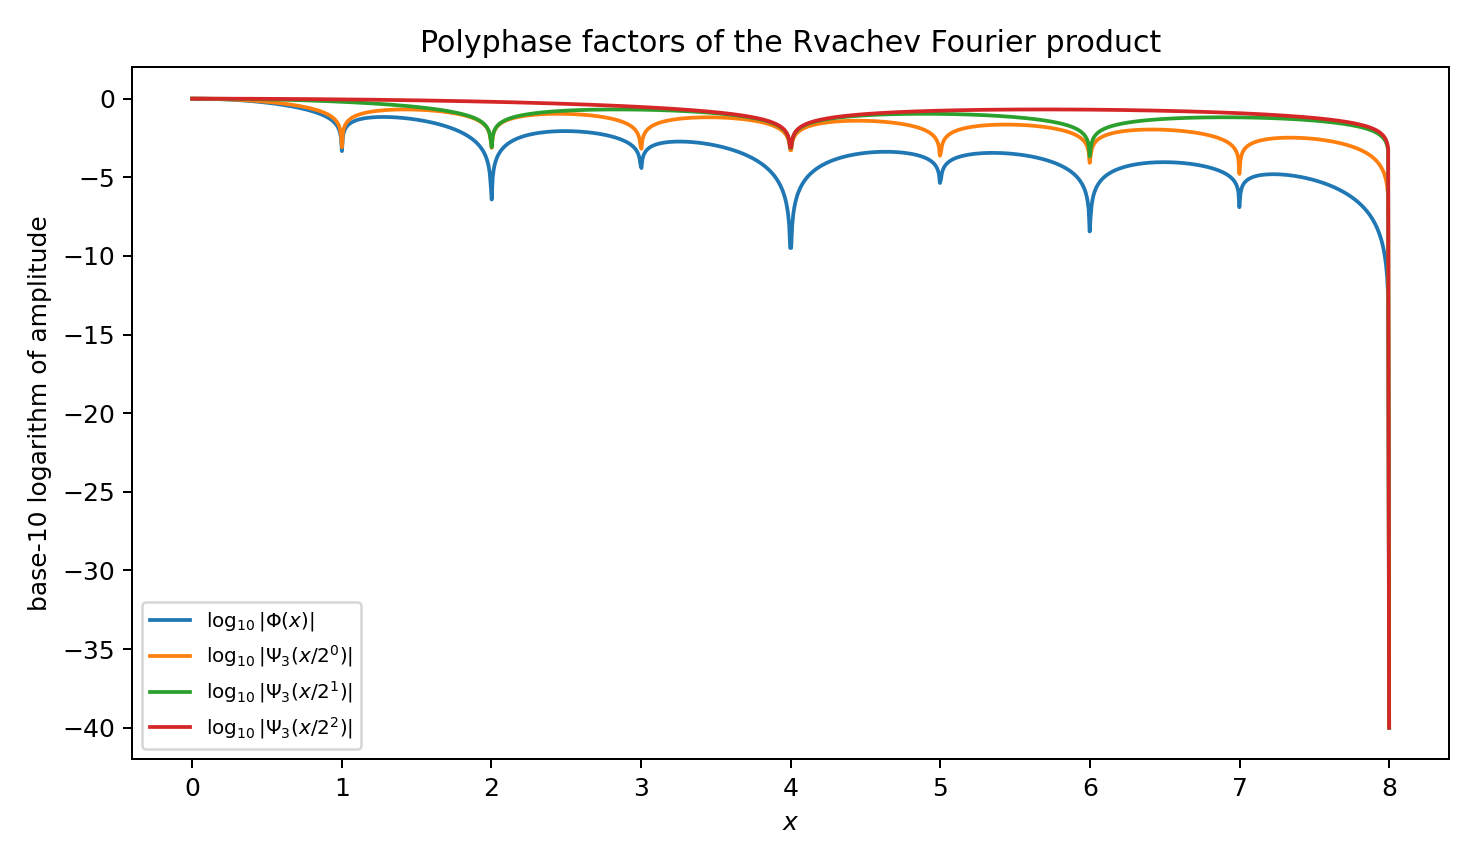
\includegraphics[width=0.97\textwidth]{polyphase_fourier_factors.png}
\caption{For $r=3$, the logarithmic magnitude of the full Fourier image and
its three sparse factors.  At each integer zero the component multiplicities
add to the multiplicity of $\Phi$.  The graph clips the logarithm near zeros;
the product identity itself was checked at high precision away from and near
the zero lattice.}
\label{fig:polyphase-factors}
\end{figure}

The jump-comb visualization in \cref{fig:TM-jump-comb} is produced from the
exact subset sums, not by differentiating noisy sampled data.  This matters:
the highest classical derivative is piecewise constant and its jumps are
mathematically exact Dirac masses in the next distributional derivative.

\subsection{Reproduction}

From the extracted archive directory, run
\begin{lstlisting}[style=python]
python numerical_experiments.py
\end{lstlisting}
The script writes
\begin{itemize}
\item \texttt{polyphase\_product\_checks.csv};
\item \texttt{fourier\_deconvolution\_checks.csv};
\item \texttt{power\_sum\_moment\_checks.csv};
\item \texttt{polyphase\_cumulant\_checks.csv};
\item \texttt{operator\_coefficients.csv};
\item the two PDF/PNG figures used in this report; and
\item \texttt{verification\_log.txt}.
\end{itemize}
No network access, random seed, or machine-dependent numerical integration is
required.

\begin{warning}
A tiny residual is not used as a proof of an infinite-product identity.  The
proofs precede the experiments.  The checks are valuable because the formulas
contain several easily misplaced factors: $2\pi$, the centered support radius,
$q^{\binom N2}$, the derivative sign $(-1)^N$, and the distinction between
$\Psi_r(q^Nz)$ and $\Psi_r(z/2^N)$.
\end{warning}

\section{Conjectures and frontier directions}
\label{sec:frontiers}

The statements in this section are separated sharply from the proved results.
Some are precise conjectures; others are research programs where fixing the
correct normalization is itself part of the work.  All concern structures
created or clarified by the polyphase decomposition.

\subsection{Uniform all-orders deconvolution}

Define coefficients $a_{r,\ell}$ by the formal identity
\begin{equation}
 \exp\!\left(-\sum_{m\ge1}c_{r,m}t^mD^{2m}\right)
 =\sum_{\ell\ge0}a_{r,\ell}t^\ell D^{2\ell}.              \label{eq:ar-ell-def}
\end{equation}
Thus
\begin{equation}
 a_{r,0}=1,
 \qquad a_{r,1}=-c_{r,1},
 \qquad a_{r,2}=-c_{r,2}+\frac{c_{r,1}^2}{2}.             \label{eq:first-ar-ell}
\end{equation}

\begin{conjecture}[Strong spline-tail expansion]
\label{conj:strong-tail}
For fixed $r,m,L\ge0$,
\begin{equation}
 \left\|D^m g_{r,N}-
   \sum_{\ell=0}^{L-1}a_{r,\ell}q^{2\ell N}
      D^{m+2\ell}g_r\right\|_{\infty}
 =\bigO_{r,m,L}(q^{2LN})                                  \label{eq:strong-tail-conj}
\end{equation}
for all sufficiently large $N$.
In particular,
\begin{equation}
 q^{-2N}(g_{r,N}^{(m)}-g_r^{(m)})
 \longrightarrow-c_{r,1}g_r^{(m+2)}                       \label{eq:first-tail-limit}
\end{equation}
uniformly.
\end{conjecture}

The local Fourier expansion proves the coefficient prediction.  A proof of the
uniform remainder must use the exact quotient
$\Psi_r(z)/\Psi_r(q^Nz)$ to control the high-frequency region where the formal
reciprocal has poles.  Compact support and superalgebraic Fourier decay make the
conjecture plausible, but the cancellation near the moving zero lattice should
be handled explicitly rather than hidden in a Taylor argument.

\subsection{Nondegeneracy of sparse Mellin harmonics}

After subtracting the elementary local and mean terms, let $P_r$ denote the
periodic fluctuation in the regularized asymptotics of $\log|\Psi_r(t)|$ or
$\log M_r(t)$.  Normalize its period to $r$:
\begin{equation}
 P_r(\theta)=\sum_{k\in\Z}c_{r,k}\e^{2\pi\ii k\theta/r}.  \label{eq:Pr-conj-Fourier}
\end{equation}

\begin{conjecture}[Mellin-harmonic nondegeneracy]
\label{conj:Mellin-nondegenerate}
Apart from coefficients forced to vanish by parity or the chosen
regularization, $c_{r,k}\ne0$ for every $k\ne0$.  Consequently the polyphase
projection
\begin{equation}
 P_1(\theta)=r\sum_{\ell\in\Z}c_{r,r\ell}\e^{2\pi\ii\ell\theta} \label{eq:Pr-projection-conj}
\end{equation}
loses harmonics only through the exact roots-of-unity cancellation of
\cref{thm:Mellin-cancellation}, not through accidental zeros of Mellin residues.
\end{conjecture}

A practical attack is to derive a rigorously convergent expression for the
regularized Mellin transform $H(s)$ and certify $H(2\pi\ii k/(r\log2))\ne0$
with interval arithmetic.  The decomposition allows one to work at the longer
period $r\log2$, where individual modes may be easier to separate numerically.

\subsection{Sparse endpoint asymptotics}

The component support radius is $A_r=1/[2(1-2^{-r})]$.  General small-deviation
heuristics for geometrically weighted sums predict
\begin{equation}
 \log g_r(A_r-t)
 \sim-\frac{(\log(1/t))^2}{2r\log2},
 \qquad t\downarrow0.                                    \label{eq:sparse-leading-endpoint}
\end{equation}
The full Rvachev endpoint theory in the corpus contains much finer lower
Lambert--$W$ and periodic structure.

\begin{conjecture}[Sparse Lambert--$W$ transseries]
\label{conj:sparse-Lambert}
For each $r\ge1$, the endpoint $g_r(A_r-t)$ has an all-orders transseries in a
lower-branch Lambert coordinate whose algebraic coefficients are accompanied
by a nonconstant periodic function of logarithmic phase with fundamental
period $r\log2$.  Under convolution of the $r$ polyphase dilates, the periodic
coefficients combine by the Mellin projector of
\cref{cor:periodic-filter} to give the ordinary period-$\log2$ Rvachev
expansion.
\end{conjecture}

This conjecture is stronger than merely replacing $\log2$ by $r\log2$ in a leading term.  The saddle location, the determinant
factor, and the phase origin must all be recomputed for $M_r$.  The reward is an
``analysis then synthesis'' derivation of the full endpoint fluctuation from
sparser components.

\subsection{Radon tomography and section algorithms}

The equality
\begin{equation}
 \cC_{w_r}p_r(2x-1)=\cR_{w_r}p_r(x-1)                      \label{eq:tomography-core}
\end{equation}
invites several geometric questions.

\begin{problem}[Direct section computation]
Develop a certified quadrature for $F$ and $G$ based on the section integral
\eqref{eq:F-section-coordinates}, compare its conditioning with direct Fourier
inversion, and determine the optimal choice of $r$ as a function of the target
point and precision.
\end{problem}

For $r=2$, the integrand is a product of two copies of a broader, flatter
component $g_2$.  Near the endpoints of $F$, a larger $r$ may distribute the
small-deviation event across a higher-dimensional section and improve numerical
stability; in the interior, the dimensional cost may dominate.  This tradeoff
is concrete and testable.

\begin{problem}[Quantile tomography]
Use
\begin{equation}
 \cC_{w_r}p_r(2G(y)-1)=\cR_{w_r}p_r(G(y)-1)=y              \label{eq:quantile-tomography-problem}
\end{equation}
to construct monotone Newton or safeguarded secant schemes in which both the
residual and derivative are computed as sections of the same product density.
Investigate whether the two-level geometry yields a posteriori error bounds
stronger than generic inverse-function estimates.
\end{problem}

\subsection{Orthogonal polynomials and sparse spectral data}

Let $(P_n^{(r)})$ be the monic orthogonal polynomials for $g_r(x)\dd x$.
Symmetry gives
\begin{equation}
 P_{n+1}^{(r)}(x)=xP_n^{(r)}(x)-\beta_n^{(r)}P_{n-1}^{(r)}(x). \label{eq:sparse-Jacobi}
\end{equation}
The moments are explicit Bell--Bernoulli expressions, so every finite
$\beta_n^{(r)}$ is an exact rational number.

\begin{problem}[Endpoint-flat Jacobi asymptotics]
Determine the asymptotic expansion of $\beta_n^{(r)}$ beyond the universal
Nevai limit $A_r^2/4$.  In particular, test whether the infinitely flat,
log-periodic endpoint behavior of $g_r$ creates logarithmic or periodic
corrections to the usual algebraic recurrence-coefficient asymptotics.
\end{problem}

The polyphase convolution gives a second route: the Jacobi data of $u$ should
be constrained by the $r$ component moment sequences and their scaled free
cumulant-like convolution algebra.  No simple formula is expected, but exact
Hankel determinants at moderate order may reveal a stable pattern.

\subsection{Twisted scale characters}

The ordinary polyphase split uses the trivial character of the cyclic group
$\Z/r\Z$.  Near the origin, where logarithms are single-valued, introduce
\begin{equation}
 L_{r,\ell}(z)=\sum_{a=0}^{r-1}\omega^{-a\ell}
 \log\Psi_r(z/2^a),
 \qquad \omega=\e^{2\pi\ii/r}.                            \label{eq:twisted-scale-log}
\end{equation}
Then $L_{r,0}=\log\Phi$, while the nontrivial $L_{r,\ell}$ isolate scale
characters which cancel in the ordinary product.

\begin{problem}[Scale-character continuation]
Find natural single-valued analytic or meromorphic objects whose local
logarithms are $L_{r,\ell}$, describe their zero divisors, and determine whether
they encode the discarded Mellin harmonics directly.  A successful construction
would diagonalize modular scale refinement in the same way that the finite
Fourier transform diagonalizes cyclic translation.
\end{problem}

Complex powers of factors cannot simply be written globally because zeros
create monodromy.  A divisor-valued or line-bundle formulation may be the right
language.

\subsection{General bases and residue subsets}

For $b>1$, the formal analogue
\begin{equation}
 \Psi_{b,r}(z)=\prod_{m\ge0}\sincpi(z/b^{rm})              \label{eq:base-b-sparse}
\end{equation}
has a base-$b$ polyphase decomposition.  Much of the generic base-$b$ theory is
already present in the corpus, so the frontier is not the definition itself.
The new questions are structural:
\begin{itemize}
\item classify residue subsets $A\subset\{0,\ldots,r-1\}$ for which the
      partial product is a characteristic function with especially simple
      compact support or refinement equation;
\item determine the lobe-sign automatic sequence when $b$ is not even, where
      the parity simplification in \eqref{eq:sparse-sign-base} changes;
\item replace binary signs by roots of unity and recover generalized
      Prouhet--Thue--Morse words from distributional derivatives of complex or
      vector-valued box splines;
\item identify the exact Mellin character projector for arbitrary scale
      residue weights.
\end{itemize}

\subsection{Arithmetic of sparse knot limits}

All finite knot locations, cumulants, moments, and power sums are rational for
$q=2^{-r}$.  The limiting density values are subtler.

\begin{problem}[Sparse-adic values]
Determine the arithmetic nature of $g_r(x)$ and its derivatives at rational
points whose denominators are powers of $2^r$.  Establish either a rationality
theorem with denominator bounds, analogous to the dyadic Fabius theory, or a
sharp obstruction showing why the self-CDF mechanism at $r=1$ is exceptional.
\end{problem}

The plateau present for $r\ge2$ supplies many trivial rational values, but the
transition regions carry the real arithmetic content.  The nested
factorization \eqref{eq:nested-gr} may transfer information between different
$r$.

\subsection{Formalization roadmap}

The new theorem chain is unusually well suited to formal verification because
most proofs reduce to finite reindexing, characteristic functions, and
polynomial distribution identities.

A practical Lean sequence is:
\begin{enumerate}
\item define $\Psi_r$ as a locally uniformly convergent entire product and
      prove the partition $n=a+rm$;
\item construct $Z_r$ from the existing weighted-uniform probability
      infrastructure and identify its characteristic function;
\item prove the finite and infinite convolution factorizations;
\item formalize zero multiplicities using $\nu_2$ and Euclidean division;
\item define $g_{r,N}$ as a finite convolution, then prove the truncated-power
      formula and $D^Ng_{r,N}$ as a finite signed measure;
\item prove the bit-reversal ordering and parity invariance;
\item derive the power-sum identity by distributional integration by parts,
      or first in the polynomial finite-difference algebra and then transfer;
\item connect finite cumulants to Bell polynomials and Bernoulli numbers;
\item formalize the base-$2^r$ lobe-sign theorem using the valuation-counting
      identity;
\item treat Radon/coarea statements last, since they require the heaviest
      measure-geometric library support.
\end{enumerate}
The finite jump and power-sum layer can be formalized without first developing
all of infinite-product complex analysis, making it a good initial target.

\begin{frontierbox}[Highest-value next experiments]
The most decisive near-term computations are: interval certification of the
first sparse Mellin harmonics; high-order exact Jacobi coefficients for
$g_r$; uniform-error measurements for \eqref{eq:strong-tail-conj}; and a direct
comparison of Fourier versus Radon-section evaluation of $F$ and $G$.  Each
experiment tests a precise structural prediction and can feed directly into a
proof attempt.
\end{frontierbox}

\section{Conclusion}
\label{sec:conclusion}

The Fabius--Rvachev system is unusually representation-rich because a single
object lies at the intersection of compactly supported smooth analysis,
probability, automatic sequences, infinite products, spectral determinants,
and digital asymptotics.  The audited repository already develops most of the
classical and several frontier realizations.  The main purpose of this report
has been to add a layer that cuts across those existing themes rather than
repeat them.

The central operation is Euclidean division of the Fourier scale index.  From
that elementary reindexing follow:
\begin{enumerate}
\item a sparse characteristic function $\Psi_r$, its compact density $g_r$,
      and a unique polyphase convolution factorization of $u$;
\item staircase cosine exponents, quotient-valued zero multiplicities,
      Gamma and canonical products, a sparse spectral zeta, exact determinant
      splitting, and cumulant recombination;
\item a roots-of-unity projector on Mellin poles and logarithmic-scale
      harmonics;
\item a product-density Radon representation in which a Fabius value is both a
      half-space volume and a parallel hyperplane section;
\item finite sparse splines whose highest derivative jumps, distributional
      derivative, Fourier quotient, and cardinal integrals all recover
      Thue--Morse signs;
\item an exact left-to-right reading of the ordinary Thue--Morse word from the
      spatially ordered jumps;
\item Bell--Bernoulli formulas for every surviving signed power sum and for the
      separate evil and odious power sums;
\item an infinite product of uniform averaging operators with an exact
      Bernoulli/zeta differential logarithm;
\item a twisted Poisson family and a zero-slope sine series for $F$;
\item a factorization of binary Thue--Morse parity into overlapping
      base-$2^r$ digit-parity characters, together with recovery from odd zero
      slopes of $\Phi$.
\end{enumerate}

Several of these statements are short once the correct object is introduced.
That is a strength rather than a weakness: the polyphase factor exposes a
common mechanism behind formulas which otherwise look unrelated.  The next
stage should combine the sparse Mellin analysis, endpoint Lambert--$W$
coordinates, and the exact finite jump calculus.  Those three layers offer a
credible route from computer-assisted experimentation to theorem-level control
of periodic asymptotics and approximation errors.

\appendix

\section{Corpus audit boundary}
\label{app:corpus}

The source boundary is the repository commit
\begin{center}
\nolinkurl{19ad531146cda7bc11a206827566db7f5753d5b3}.
\end{center}
The branch advanced while the audit was in progress; pinning the hash prevents
later reorganizations from silently changing the novelty comparison.

The recursive inventory covered current expositions, the living frontier
synthesis, active thematic drafts, frozen archive lineages, and corrected
paper sources.  The principal exclusion documents were:
\begin{center}
\small
\begin{tabularx}{0.96\textwidth}{@{}p{0.32\textwidth}X@{}}
\toprule
Corpus component & Main themes excluded from novelty claims\\
\midrule
Primary exposition & Characterization, probability, Fourier product, dyadic values, derivatives, partition of unity, arithmetic.\\
Thue--Morse atlas & Signed/unsigned formulas, automatic and Mahler forms, binomial and valuation formulas, Prouhet identities, rarefied sums.\\
Finite-block frontier & Exact tails, confluent cancellation, finite products, extrapolation, spline approximants.\\
Representation frontier & Resolvents, logarithmic fixed points, Jacobi fractions, determinants, transform families.\\
Multiresolution report & Haar, Walsh, Faber--Schauder, beta and sinc mixtures, rational finite systems.\\
Inverse/sampling report & Quantile transport, inverse self-sampling, level-set and transform formulas.\\
Exponent/$q$ report & Newton exponent sequences, Gaussian $q$-binomial structure, Bell and Bernoulli coefficient algebra.\\
Spectral/arithmetic report & Zero jets, spectral zeta and determinants, half-integer spectra, arithmetic rays.\\
Integration reports & Integer/fractional transforms, repeated antiderivatives, monomial products, inverse integrals.\\
Fourier-decay campaign & Sharp decay scales, orbit dependence, log-periodic fluctuations, audit of competing asymptotics.\\
\bottomrule
\end{tabularx}
\end{center}

The label \statusnew therefore means ``not located in this pinned TeX corpus
after targeted full-tree searches.''  It is not a claim that no equivalent
formula has ever appeared in the worldwide literature.  Targeted public-web
searches for the exact combinations ``polyphase Rvachev'', ``scale-residue sinc
factorization'', ``Thue--Morse box-spline jumps'', and ``Fabius hyperplane
section'' did not reveal a direct antecedent, but a formal priority claim would
require a dedicated bibliographic study across several adjacent literatures.

\section{Archive contents and reproducibility}
\label{app:archive}

The ZIP archive accompanying this report contains:
\begin{itemize}
\item \texttt{fabius\_rvachev\_polyphase\_representations.tex}, the source;
\item \texttt{fabius\_rvachev\_polyphase\_representations.pdf}, the rendered report;
\item \texttt{numerical\_experiments.py}, with detailed comments and no network dependency;
\item five CSV verification tables;
\item two figures in both PNG and PDF form;
\item \texttt{verification\_log.txt};
\item \texttt{README.md} with build commands; and
\item \texttt{MANIFEST.sha256} for integrity checking.
\end{itemize}

A standard build is
\begin{lstlisting}[style=python]
python numerical_experiments.py
latexmk -pdf -interaction=nonstopmode \
  fabius_rvachev_polyphase_representations.tex
\end{lstlisting}
The report itself does not require rerunning the experiments if the included
figures are retained.

\section{Selected identities in machine-friendly form}
\label{app:machine-identities}

For use in symbolic systems, the main new identities can be summarized without
prose as follows.  Put $q=2^{-r}$.
\begin{align}
 \Psi_r(z)&=\prod_{m\ge0}\sincpi(q^mz),                    \label{eq:machine-1}\\
 \Phi(z)&=\prod_{a=0}^{r-1}\Psi_r(2^{-a}z),                \label{eq:machine-2}\\
 \log\Psi_r(z)&=-\sum_{m\ge1}\frac{\zeta(2m)}{m(1-q^{2m})}z^{2m}, \label{eq:machine-3}\\
 \ord_{z=n}\Psi_r&=1+\left\lfloor\frac{\nu_2(n)}r\right\rfloor, \label{eq:machine-4}\\
 \mathcal Z_r(s)&=\frac{\zeta(s)}{1-2^{-rs}},             \label{eq:machine-5}\\
 g_{r,N}(x)&=\frac{q^{-\binom N2}}{(N-1)!}
 \sum_{k<2^N}\eps_k(x-x_{r,N,k})_+^{N-1},                \label{eq:machine-6}\\
 D^Ng_{r,N}&=q^{-\binom N2}\sum_{k<2^N}\eps_k\delta_{x_{r,N,k}}, \label{eq:machine-7}\\
 \eps_k&=q^{\binom N2}[D^{N-1}g_{r,N}]_{x_{r,N,k}},       \label{eq:machine-8}\\
 \widehat{g_{r,N}}(z)&=\Psi_r(z)/\Psi_r(q^Nz),            \label{eq:machine-9}\\
 \sum_{k<2^N}\eps_kx_{r,N,k}^{N+m}
 &=(-1)^Nq^{\binom N2}\frac{(N+m)!}{m!}\mu_m^{(r,N)},    \label{eq:machine-10}\\
 \eps_n&=\prod_{a=0}^{r-1}(-1)^{s_{2^r}(\lfloor n/2^a\rfloor)}, \label{eq:machine-11}\\
 \eps_n&=-\sgn\Phi'(2n+1).                               \label{eq:machine-12}
\end{align}
These formulas use the Fourier convention \eqref{eq:Fourier-convention}; a
computer algebra implementation using another convention must modify every
$2\pi$ factor consistently.

\begingroup
\small
\begin{thebibliography}{99}

\bibitem{jessen1935}
B.~Jessen and A.~Wintner,
\newblock Distribution functions and the Riemann zeta function,
\newblock \emph{Transactions of the American Mathematical Society} 38 (1935),
48--88.
\newblock DOI: \href{https://doi.org/10.1090/S0002-9947-1935-1501802-5}{10.1090/S0002-9947-1935-1501802-5}.

\bibitem{fabius1966}
J.~Fabius,
\newblock A probabilistic example of a nowhere analytic $C^\infty$-function,
\newblock \emph{Zeitschrift f\"ur Wahrscheinlichkeitstheorie und Verwandte
Gebiete} 5 (1966), 173--174.
\newblock DOI: \href{https://doi.org/10.1007/BF00536652}{10.1007/BF00536652}.

\bibitem{arias1982}
J.~Arias de Reyna,
\newblock Definici\'on y estudio de una funci\'on indefinidamente diferenciable
de soporte compacto,
\newblock \emph{Revista de la Real Academia de Ciencias Exactas, F\'isicas y
Naturales} 76(1) (1982), 21--38.
\newblock English translation: \href{https://arxiv.org/abs/1702.05442}{arXiv:1702.05442}.

\bibitem{arias2018}
J.~Arias de Reyna,
\newblock Arithmetic of the Fabius function,
\newblock \href{https://arxiv.org/abs/1702.06487}{arXiv:1702.06487}, 2017.

\bibitem{rvachev1990}
V.~A.~Rvachev,
\newblock Compactly supported solutions of functional-differential equations
and their applications,
\newblock \emph{Russian Mathematical Surveys} 45(1) (1990), 87--120.
\newblock DOI: \href{https://doi.org/10.1070/RM1990v045n01ABEH002324}{10.1070/RM1990v045n01ABEH002324}.

\bibitem{flajolet1995}
P.~Flajolet, X.~Gourdon, and P.~Dumas,
\newblock Mellin transforms and asymptotics: harmonic sums,
\newblock \emph{Theoretical Computer Science} 144 (1995), 3--58.
\newblock DOI: \href{https://doi.org/10.1016/0304-3975(95)00002-E}{10.1016/0304-3975(95)00002-E}.

\bibitem{corless1996}
R.~M.~Corless, G.~H.~Gonnet, D.~E.~G.~Hare, D.~J.~Jeffrey, and D.~E.~Knuth,
\newblock On the Lambert $W$ function,
\newblock \emph{Advances in Computational Mathematics} 5 (1996), 329--359.
\newblock DOI: \href{https://doi.org/10.1007/BF02124750}{10.1007/BF02124750}.

\bibitem{allouche2003}
J.-P.~Allouche and J.~Shallit,
\newblock \emph{Automatic Sequences: Theory, Applications, Generalizations},
\newblock Cambridge University Press, 2003.

\bibitem{aistleitner2017}
C.~Aistleitner, R.~Hofer, and G.~Larcher,
\newblock On evil Kronecker sequences and lacunary trigonometric products,
\newblock \emph{Annales de l'Institut Fourier} 67(2) (2017), 637--687.
\newblock DOI: \href{https://doi.org/10.5802/aif.3094}{10.5802/aif.3094}.

\bibitem{repoPrimary}
V.~Reshetnikov,
\newblock \emph{Fabius Function and Rvachev Up-Function}, living TeX synthesis,
\newblock \repo, pinned commit
\nolinkurl{19ad531146cda7bc11a206827566db7f5753d5b3}.
\newblock \url{https://github.com/VladimirReshetnikov/ProveIt/blob/19ad531146cda7bc11a206827566db7f5753d5b3/Analysis/FabiusFunction/docs/Fabius_Function_and_Rvachev_Up/Fabius_Function_and_Rvachev_Up.tex}.

\bibitem{repoAtlas}
V.~Reshetnikov,
\newblock \emph{Thue--Morse Formula Atlas},
\newblock \repo, pinned commit
\nolinkurl{19ad531146cda7bc11a206827566db7f5753d5b3}.
\newblock \url{https://github.com/VladimirReshetnikov/ProveIt/blob/19ad531146cda7bc11a206827566db7f5753d5b3/Analysis/FabiusFunction/docs/non-formalized-research-frontiers/drafts/thue-morse/Thue_Morse_Formula_Atlas/Thue_Morse_Formula_Atlas.tex}.

\bibitem{repoFiniteBlock}
V.~Reshetnikov,
\newblock \emph{Fabius--Rvachev--Thue--Morse Frontier Results}, finite-block and
confluent calculus report,
\newblock \repo, pinned commit
\nolinkurl{19ad531146cda7bc11a206827566db7f5753d5b3}.
\newblock \url{https://github.com/VladimirReshetnikov/ProveIt/blob/19ad531146cda7bc11a206827566db7f5753d5b3/Analysis/FabiusFunction/docs/non-formalized-research-frontiers/drafts/thue-morse/Fabius_Rvachev_Thue_Morse_Frontier_Results/Fabius_Rvachev_Thue_Morse_Frontier_Results.tex}.

\bibitem{repoRepresentations}
V.~Reshetnikov,
\newblock \emph{Fabius--Rvachev Representation Frontiers},
\newblock \repo, pinned commit
\nolinkurl{19ad531146cda7bc11a206827566db7f5753d5b3}.
\newblock \url{https://github.com/VladimirReshetnikov/ProveIt/blob/19ad531146cda7bc11a206827566db7f5753d5b3/Analysis/FabiusFunction/docs/non-formalized-research-frontiers/drafts/representations/Fabius_Rvachev_Representation_Frontiers/rvachev_fabius_representation_frontiers.tex}.

\bibitem{repoMultiresolution}
V.~Reshetnikov,
\newblock \emph{Fabius--Rvachev Multiresolution Report},
\newblock \repo, pinned commit
\nolinkurl{19ad531146cda7bc11a206827566db7f5753d5b3}.
\newblock \url{https://github.com/VladimirReshetnikov/ProveIt/blob/19ad531146cda7bc11a206827566db7f5753d5b3/Analysis/FabiusFunction/docs/non-formalized-research-frontiers/drafts/representations/Fabius_Rvachev_Multiresolution_Report/fabius_rvachev_multiresolution_report.tex}.

\bibitem{repoInverse}
V.~Reshetnikov,
\newblock \emph{Inverse and Sampling Frontiers},
\newblock \repo, pinned commit
\nolinkurl{19ad531146cda7bc11a206827566db7f5753d5b3}.
\newblock \url{https://github.com/VladimirReshetnikov/ProveIt/blob/19ad531146cda7bc11a206827566db7f5753d5b3/Analysis/FabiusFunction/docs/non-formalized-research-frontiers/drafts/inverse-and-sampling/Inverse_and_Sampling_Frontiers/Inverse_and_Sampling_Frontiers.tex}.

\bibitem{repoExponents}
V.~Reshetnikov,
\newblock \emph{Exponents and $q$-Series Frontiers},
\newblock \repo, pinned commit
\nolinkurl{19ad531146cda7bc11a206827566db7f5753d5b3}.
\newblock \url{https://github.com/VladimirReshetnikov/ProveIt/blob/19ad531146cda7bc11a206827566db7f5753d5b3/Analysis/FabiusFunction/docs/non-formalized-research-frontiers/drafts/exponents-and-q-series/Exponents_and_q_Series_Frontiers/Exponents_and_q_Series_Frontiers.tex}.

\bibitem{repoSpectra}
V.~Reshetnikov,
\newblock \emph{Spectra and Arithmetic Frontiers},
\newblock \repo, pinned commit
\nolinkurl{19ad531146cda7bc11a206827566db7f5753d5b3}.
\newblock \url{https://github.com/VladimirReshetnikov/ProveIt/blob/19ad531146cda7bc11a206827566db7f5753d5b3/Analysis/FabiusFunction/docs/non-formalized-research-frontiers/drafts/spectra-and-arithmetic/Spectra_and_Arithmetic_Frontiers/Spectra_and_Arithmetic_Frontiers.tex}.

\end{thebibliography}
\endgroup

\end{document}
